\documentclass[preprint,10pt]{elsarticle}

% Vector fonts with a Unicode map, so that PDF text extraction (and journal checkers)
% read ligatures such as fi/fl correctly instead of Type 3 bitmaps.
\input{glyphtounicode}
\pdfgentounicode=1
\usepackage[T1]{fontenc}
\usepackage{lmodern}

\usepackage{amsmath,amssymb}
\usepackage{graphicx}
\usepackage{booktabs}
\usepackage{tabularx}
\usepackage{array}
\usepackage{xcolor}
\usepackage{url}
\usepackage{enumitem}
\usepackage{algorithm}
\usepackage{algorithmic}
\usepackage{tikz}
\usetikzlibrary{positioning,arrows.meta,fit,backgrounds}
\usepackage{pgfplots}
\pgfplotsset{compat=1.18}
\newif\ifshoworacle
\showoracletrue % set \showoraclefalse to hide Selection-Matched values in the new figures
\usepackage[hidelinks]{hyperref}

% Document formatting adjustments for academic readability and clean float placement
\setlength{\emergencystretch}{3em}
\renewcommand{\topfraction}{0.9}
\renewcommand{\bottomfraction}{0.8}
\renewcommand{\textfraction}{0.07}
\renewcommand{\floatpagefraction}{0.75}
\setcounter{totalnumber}{4}
\setlength{\abovecaptionskip}{4pt}
\setlength{\belowcaptionskip}{2pt}
\setlength{\textfloatsep}{8pt plus 1pt minus 2pt}
\setlength{\intextsep}{6pt plus 1pt minus 1pt}
\setlength{\abovedisplayskip}{4pt plus 1pt minus 1pt}
\setlength{\belowdisplayskip}{4pt plus 1pt minus 1pt}

\journal{Natural Language Processing Journal}

\begin{document}

\newcommand{\nVerified}{40}
\newcommand{\nTotal}{40}
\newcommand{\graphSteps}{44}
\newcommand{\graphRootNodes}{7}
\newcommand{\keyFactRecallNaive}{0.712}
\newcommand{\stepCoverageNaive}{0.727}
\newcommand{\refusalAccuracyNaive}{0.600}
\newcommand{\keyFactRecallGraph}{0.698}
\newcommand{\stepCoverageGraph}{0.687}
\newcommand{\refusalAccuracyGraph}{0.600}
\newcommand{\keyFactRecallWorkflow}{0.955}
\newcommand{\stepCoverageWorkflow}{1.000}
\newcommand{\refusalAccuracyWorkflow}{1.000}
\newcommand{\keyFactRecallFullContext}{0.962}
\newcommand{\stepCoverageFullContext}{0.944}
\newcommand{\refusalAccuracyFullContext}{1.000}
\newcommand{\judgeModel}{llama3.1:8b}



\begin{frontmatter}

\title{Procedure Selection versus Workflow Structuring in Local RAG for Institutional SOP Question Answering: An Ablation Study}

\author[undip]{Cipta Fikri Wiratama}
\ead{fikriw@students.undip.ac.id}

\author[undip]{Indra Waspada\corref{cor1}}
\ead{indrawaspada@lecturer.undip.ac.id}

\author[undip]{Dhena Kamalia Fu'adi}

\author[usm]{Ramona Ramli\corref{cor1}}
\ead{ramona@usm.my}

\author[undip]{Henri Tantyoko}

\author[undip]{Sandy Kurniawan}

\author[undip]{Satriawan Rasyid Purnama}

\cortext[cor1]{Corresponding author}

\affiliation[undip]{organization={Department of Informatics, Faculty of Science and Mathematics, Universitas Diponegoro},
            city={Semarang},
            postcode={50275},
            country={Indonesia}}

\affiliation[usm]{organization={School of Computer Sciences, Universiti Sains Malaysia},
            city={Pulau Pinang},
            postcode={11800 USM},
            country={Malaysia}}

\begin{abstract}
\textbf{Background:} Standard operating procedures (SOPs) in university administration require answers that preserve step order, responsible actors, and required documents, yet locally hosted small language models are easily distracted by passages from lexically overlapping procedures.

\textbf{Methods:} We pair rule-based procedure selection with directed workflow graphs that encode chronological steps and responsible actors (Workflow GraphRAG). We compare it with nine configurations, including a selection-matched ablation that supplies the same selected SOP as raw text, on a verified 40-question benchmark over seven Indonesian institutional SOPs, using a local generator (\texttt{gemma4:e2b}, 5.1B parameters).

\textbf{Results:} Workflow GraphRAG achieves 0.955 key-fact recall (KFR) and 1.000 step coverage, above naive RAG (0.712 KFR; Holm-adjusted $p=0.053$) and a custom entity-graph baseline (0.698 KFR; Holm-adjusted $p=0.034$). The selection-matched ablation reaches 0.962 KFR, and a paired Wilcoxon test detects no recall advantage from graph serialization ($p=0.59$). Non-fine-tuned base embeddings raise naive RAG to 0.910 KFR. Workflow GraphRAG shows no topological inversions ($\text{TIR}=0.000$), unlike entity-graph retrieval ($\text{TIR}=0.083$) and full-context prompting ($\text{TIR}=0.027$), and uses 44\% fewer prompt tokens than full-context prompting at comparable recall.

\textbf{Conclusions:} Procedure-level selection is the primary driver of factual recall in concise procedural corpora, while workflow graphs provide chronological formatting integrity and token efficiency.
\end{abstract}

\begin{keyword}
Retrieval-augmented generation \sep GraphRAG \sep Standard operating procedures \sep Workflow representation \sep Small language models \sep Ablation study \sep Evaluation metrics
\end{keyword}

\end{frontmatter}

\noindent{\small\textit{Word count:} 7,303 words including references (6,566 excluding references).}\par

%% ===================================================================
\section{Introduction}
\label{sec:intro}

Universities run routine student services, such as academic leave, course registration, tuition postponement, and credential legalisation, through Standard Operating Procedures (SOPs). Staff spend substantial time answering repeated questions about their steps, responsible units, and prerequisites, which makes question answering with Large Language Models (LLMs) attractive.

Cloud-hosted models, however, add per-query costs and expose student data to third parties. Small open-weights models (2B to 5B parameters) running locally avoid both problems but are more easily distracted by irrelevant context \cite{liu2024lost}. In administrative answers this matters: a transposed step, a wrong official, or an omitted form sends a student to the wrong desk.

Retrieval-Augmented Generation (RAG) grounds generation in retrieved passages \cite{lewis2020rag,gao2023ragsurvey}. Short SOPs become whole-document chunks, so top-$k$ retrieval returns several SOPs that share vocabulary (e.g., Dean, Academic Office, verification, signatures), and the generator must separate competing procedures, risking cross-contamination and wrong step order. Graph-based RAG \cite{peng2024graphragsurvey,pan2024unifying} mostly builds entity-relation graphs \cite{edge2024graphrag,guo2024lightrag,gutierrez2024hipporag}, which do not encode execution order or step-level responsibility.

We investigate \emph{Process-Aware Workflow GraphRAG}, which models each SOP as a directed workflow graph \cite{dumas2018fundamentals} whose step nodes record the performing actor, action, required documents, and deliverables; a rule-based selector picks the target SOP, and its ordered steps plus supporting chunks are passed to a local generator (\texttt{gemma4:e2b}). Gains from graph-enhanced retrieval are often credited to the graph without testing whether they come from \emph{retrieving the correct document} or from \emph{presenting it as a graph}. We therefore ask four research questions:
\begin{itemize}[leftmargin=*]
\item \textbf{RQ1 (Answer quality):} How does the workflow-aware pipeline compare with chunk retrieval and an entity-graph baseline in factual completeness, step coverage, and order and actor correctness?
\item \textbf{RQ2 (Selection vs.\ structuring):} What does graph-derived workflow structuring add beyond selecting the same SOP and supplying its original text?
\item \textbf{RQ3 (Refusal):} How do the systems behave on out-of-scope or unanswerable questions, and which mechanisms govern their refusals?
\item \textbf{RQ4 (Efficiency):} What are the prompt-token and latency trade-offs relative to retrieval baselines and full-context prompting?
\end{itemize}

This study makes four contributions:
\begin{enumerate}[leftmargin=*]
\item \textbf{Workflow-aware procedural RAG pipeline:} rule-based SOP identification with directed workflow-graph serialization for a small local generator.
\item \textbf{Selection-versus-structure ablation:} \emph{Selection-Matched Text RAG} (logged as \emph{SOP-Oracle RAG}), which keeps selection and supporting retrieval fixed but replaces the workflow block with raw SOP text.
\item \textbf{Deterministic procedural metrics:} LLM-free Topological Inversion Rate (TIR) and Actor Mismatch Rate (AMR), used with step coverage and key-fact recall (KFR) and checked by a manual audit of 60 sampled rows.
\item \textbf{Controlled comparison:} 10 systems on a verified 40-question benchmark, showing that the ablation matches Workflow GraphRAG (0.962 vs.\ 0.955 KFR; paired Wilcoxon $p=0.59$) and that embedding configuration strongly affects standard RAG.
\end{enumerate}

%% ===================================================================
\section{Related work}
\label{sec:related}

\subsection{Retrieval-augmented generation}
RAG conditions generation on retrieved documents \cite{lewis2020rag}. Naive RAG injects the top-$k$ dense-retrieved chunks \cite{gao2023ragsurvey}; hybrid retrieval adds BM25 \cite{robertson2009bm25} with reciprocal rank fusion \cite{cormack2009rrf}; ReAct \cite{yao2023react} interleaves reasoning with search; and CRAG \cite{yan2024crag} and Self-RAG \cite{asai2024selfrag} grade evidence and rewrite queries when it is weak. All pass unstructured prose to the generator, leaving step order and actor attribution implicit. Long-context prompting avoids retrieval but raises token cost and weakens attention to mid-context content \cite{liu2024lost}.

\subsection{Graph-based RAG architectures}
Graph-based RAG adds explicit relations between pieces of evidence \cite{peng2024graphragsurvey,pan2024unifying}: Microsoft GraphRAG \cite{edge2024graphrag} summarises communities of LLM-extracted entities, LightRAG \cite{guo2024lightrag} indexes entities and relations at two levels, and HippoRAG \cite{gutierrez2024hipporag} runs Personalized PageRank over entity graphs. These graphs encode entity triples, with no notion of precedence, branching, or execution state.

\subsection{Process modelling and procedural representation}
Business Process Management models procedures as directed workflows \cite{dumas2018fundamentals}; BPMN adds actor swimlanes and branching gateways \cite{omg2011bpmn}, and process models can be extracted from text \cite{friedrich2011process}. We use workflow graphs not for simulation or compliance checking but as a retrieval and prompt-structuring substrate.

\subsection{Emerging order-aware and procedural RAG}
SOPRAG \cite{lin2026sedrag} retrieves industrial SOPs with flow-graph and entity-graph experts, and Order-Aware Hypergraph RAG \cite{wu2026okhrag} models transitions over hyperedges. Both use learned indexing at scale, and neither separates the effect of selecting the right procedure from that of structuring it; we isolate this for small local models over institutional workflows. Table~\ref{tab:positioning} contrasts the context units each method family passes to the generator.

\begin{table}[!htbp]
\centering
\caption{Structural characteristics of context units provided to the generator across retrieval paradigms. ``Implicit'' denotes that information is present in prose but requires model inference.}
\label{tab:positioning}
\small
\begin{tabularx}{\textwidth}{>{\raggedright\arraybackslash}p{3.2cm} >{\raggedright\arraybackslash}X >{\raggedright\arraybackslash}p{2.1cm} >{\raggedright\arraybackslash}p{2.1cm}}
\toprule
Method family & Context unit passed to generator & Step sequence & Actor per step \\
\midrule
Naive / Hybrid / Agentic / CRAG \cite{lewis2020rag,cormack2009rrf,yao2023react,yan2024crag} & Unstructured text chunks & Implicit & Implicit \\
Entity-graph GraphRAG \cite{edge2024graphrag,guo2024lightrag} & Entity-relation triples \& text & Not represented & Relational triples \\
Workflow GraphRAG (this work) & Directed workflow block \& chunks & Explicit & Explicit \\
Selection-Matched Text (ablation) & Whole selected SOP text \& chunks & Implicit & Implicit \\
\bottomrule
\end{tabularx}
\end{table}

%% ===================================================================
\section{Problem setting and procedural error classes}
\label{sec:problem}

\subsection{Institutional SOP corpus}
The corpus is the complete set of student-service SOPs published by the Faculty of Science and Mathematics (FSM), Universitas Diponegoro (Table~\ref{tab:corpus}): 7 one-page Indonesian documents with 44 numbered steps (about 1,097 words), each a strictly linear sequence without gateways or branches. All share one layout (Figure~\ref{fig:sopdoc}): a title, a purpose sentence that may state the maximum processing time, and numbered steps whose grammatical subject is the performing role, optionally followed by \emph{Waktu} (time), \emph{Dokumen yang dibutuhkan} (documents), and \emph{Output} lines.

\begin{table}[!htbp]
\centering
\caption{Characteristics of the 7 FSM Universitas Diponegoro SOP documents. ``PDF steps'' denotes numbered steps in official source documents; ``Graph steps'' denotes nodes in the curated workflow graph.}
\label{tab:corpus}
\small
\setlength{\tabcolsep}{4pt}
\resizebox{\linewidth}{!}{%
\begin{tabular}{lrrrr}
\toprule
SOP Document & PDF steps & Graph steps & Characters & Words \\
\midrule
Academic leave (Cuti Akademik) & 8 & 8 & 1,573 & 205 \\
Reactivation after leave (Aktif Kembali) & 3 & 3 & 597 & 84 \\
Diploma/transcript legalisation (Legalisir) & 6 & 6 & 1,640 & 208 \\
Course registration (Pengisian IRS) & 6 & 6 & 1,189 & 163 \\
Late tuition payment (Keterlambatan UKT) & 11 & 11 & 1,415 & 173 \\
Scholarship recommendation (Beasiswa) & 5 & 5 & 1,130 & 142 \\
Student activity proposal (Proposal Ormawa) & 5 & 5 & 997 & 122 \\
\midrule
Total & 44 & 44 & 8,541 & 1,097 \\
\bottomrule
\end{tabular}%
}
\end{table}

\begin{figure}[!htbp]
\centering
\resizebox{\textwidth}{!}{%
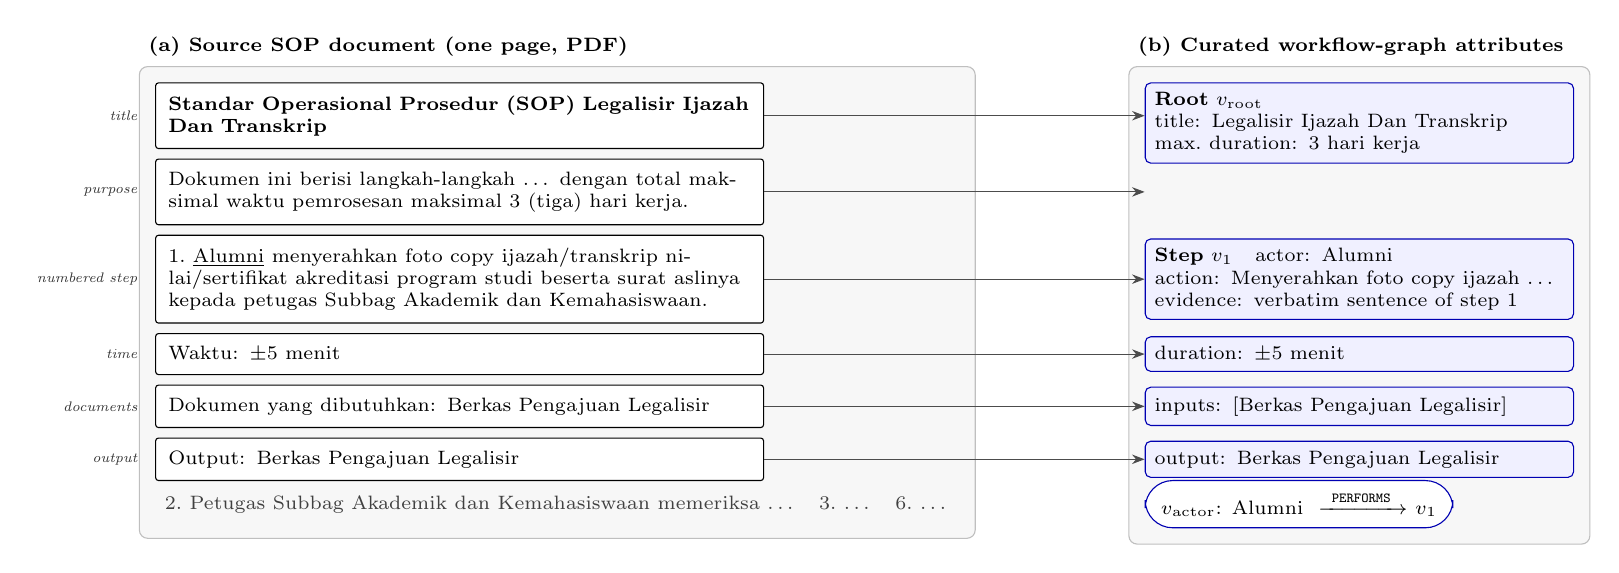
\begin{tikzpicture}[
  doc/.style={draw, fill=white, font=\scriptsize, align=left, inner sep=1.6mm, rounded corners=1pt},
  fld/.style={draw=blue!70!black, fill=blue!6, rounded corners=2pt, font=\scriptsize, align=left, inner sep=1.2mm, text width=52mm},
  tag/.style={font=\tiny\itshape, text=gray!40!black, anchor=east},
  map/.style={-{Stealth[length=1.6mm]}, gray!60!black, thin}
]
% ---------- left: the PDF page ----------
\node[doc, text width=74mm] (title) at (0,0)
  {\textbf{Standar Operasional Prosedur (SOP) Legalisir Ijazah Dan Transkrip}};
\node[doc, text width=74mm, anchor=north] (purp) at ([yshift=-1.2mm]title.south)
  {Dokumen ini berisi langkah-langkah \dots\ dengan total maksimal waktu pemrosesan maksimal 3 (tiga) hari kerja.};
\node[doc, text width=74mm, anchor=north] (step) at ([yshift=-1.2mm]purp.south)
  {1.\ \underline{Alumni} menyerahkan foto copy ijazah/transkrip nilai/sertifikat akreditasi program studi beserta surat aslinya kepada petugas Subbag Akademik dan Kemahasiswaan.};
\node[doc, text width=74mm, anchor=north] (wkt) at ([yshift=-1.2mm]step.south) {Waktu: $\pm$5 menit};
\node[doc, text width=74mm, anchor=north] (dok) at ([yshift=-1.2mm]wkt.south) {Dokumen yang dibutuhkan: Berkas Pengajuan Legalisir};
\node[doc, text width=74mm, anchor=north] (out) at ([yshift=-1.2mm]dok.south) {Output: Berkas Pengajuan Legalisir};
\node[font=\scriptsize, anchor=north west, text=gray!50!black] (more) at ([yshift=-0.6mm]out.south west) {2.\ Petugas Subbag Akademik dan Kemahasiswaan memeriksa \dots\quad 3.\ \dots\quad 6.\ \dots};
\node[tag] at ([xshift=-1mm]title.west) {title};
\node[tag] at ([xshift=-1mm]purp.west) {purpose};
\node[tag] at ([xshift=-1mm]step.west) {numbered step};
\node[tag] at ([xshift=-1mm]wkt.west) {time};
\node[tag] at ([xshift=-1mm]dok.west) {documents};
\node[tag] at ([xshift=-1mm]out.west) {output};
\begin{scope}[on background layer]
\node[draw=gray!50, fill=gray!6, rounded corners=3pt, inner sep=2mm, fit=(title)(more)] (page) {};
\end{scope}
\node[font=\scriptsize\bfseries, anchor=south west] at (page.north west) {(a) Source SOP document (one page, PDF)};
% ---------- right: graph attributes ----------
\node[fld, anchor=north west] (r1) at (8.7,0 |- title.north) {\textbf{Root} $v_{\text{root}}$\\ title: Legalisir Ijazah Dan Transkrip\\ max.\ duration: 3 hari kerja};
\node[fld, anchor=west] (s1) at (8.7,0 |- step.west) {\textbf{Step} $v_1$\quad actor: Alumni\\ action: Menyerahkan foto copy ijazah \dots\\ evidence: verbatim sentence of step 1};
\node[fld, anchor=west] (s2) at (8.7,0 |- wkt.west) {duration: $\pm$5 menit};
\node[fld, anchor=west] (s3) at (8.7,0 |- dok.west) {inputs: [Berkas Pengajuan Legalisir]};
\node[fld, anchor=west] (s4) at (8.7,0 |- out.west) {output: Berkas Pengajuan Legalisir};
\node[draw=blue!70!black, fill=white, rounded corners=3.5mm, font=\scriptsize, inner xsep=2mm, minimum height=6mm, anchor=west] (act) at (8.7,0 |- more.west) {$v_{\text{actor}}$: Alumni \ $\xrightarrow{\ \texttt{PERFORMS}\ }$\ $v_1$};
\begin{scope}[on background layer]
\node[draw=gray!50, fill=gray!6, rounded corners=3pt, inner sep=2mm, fit=(r1)(act)] (gph) {};
\end{scope}
\node[font=\scriptsize\bfseries, anchor=south west] at (gph.north west) {(b) Curated workflow-graph attributes};
% ---------- mapping arrows ----------
\draw[map] (title.east) -- (r1.west |- title.east);
\draw[map] (purp.east) -- (r1.west |- purp.east);
\draw[map] (step.east) -- (s1.west);
\draw[map] (wkt.east) -- (s2.west);
\draw[map] (dok.east) -- (s3.west);
\draw[map] (out.east) -- (s4.west);
\end{tikzpicture}}
\caption{Anatomy of an FSM SOP document and its mapping to workflow-graph attributes, shown for step 1 of the legalisation SOP. The underlined grammatical subject becomes the performing actor, the optional \emph{Waktu}, \emph{Dokumen yang dibutuhkan}, and \emph{Output} lines become duration, input, and output attributes, and the step sentence is stored verbatim as evidence.}
\label{fig:sopdoc}
\end{figure}

The steps are performed by 15 roles from the student to the university level (Figure~\ref{fig:actors}). Students perform 21 of the 44 steps in six of the seven SOPs, and several faculty roles act in more than one procedure, so SOPs share actors as well as vocabulary.

\begin{figure}[!htbp]
\centering
\resizebox{\textwidth}{!}{%
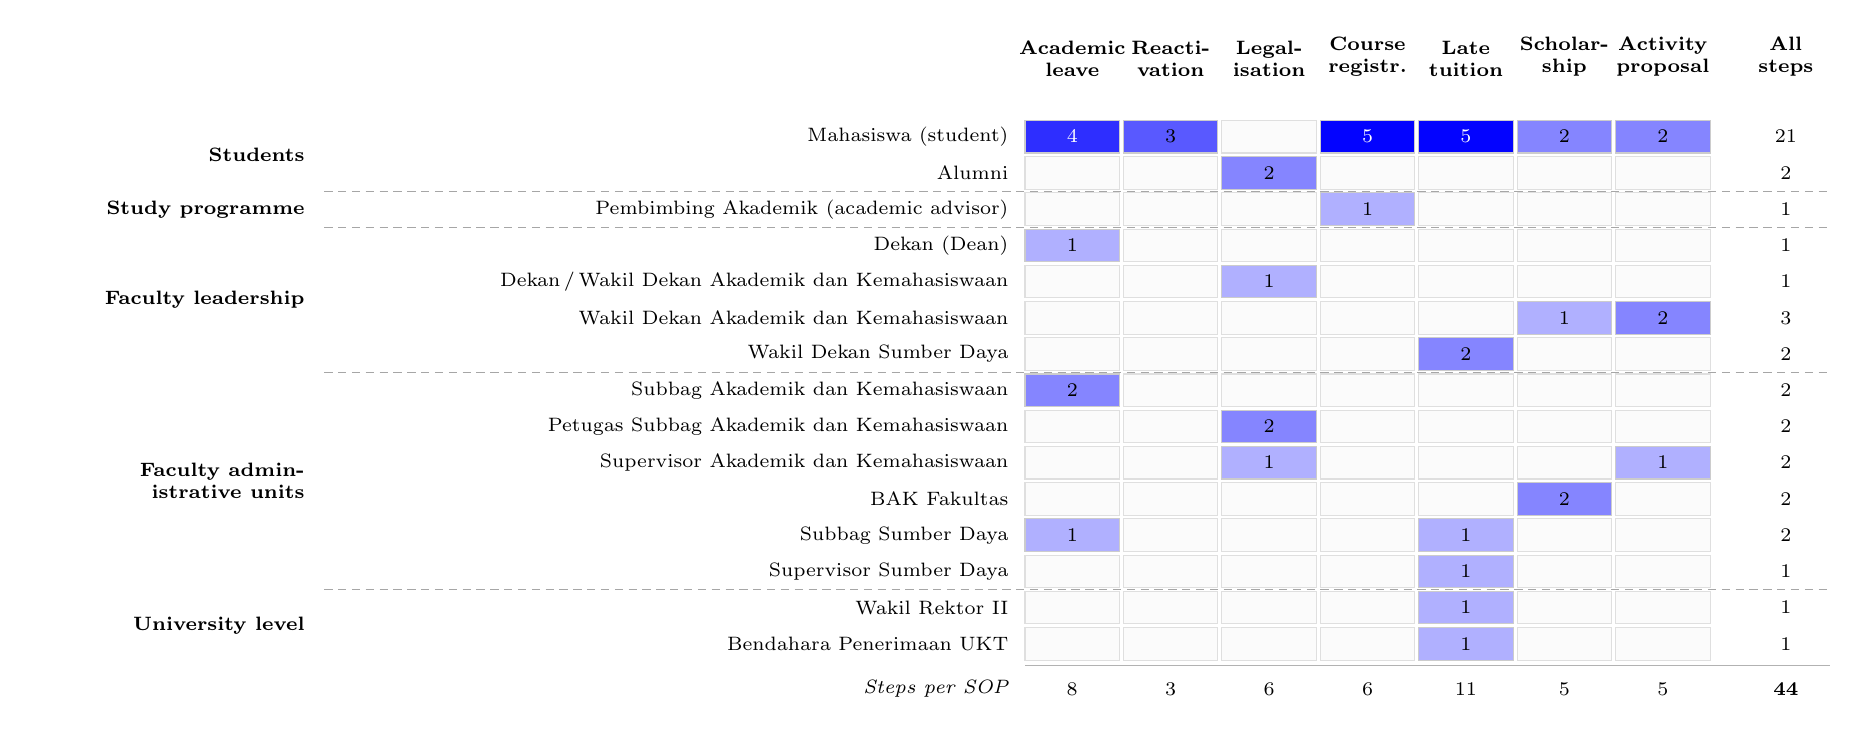
\begin{tikzpicture}[x=12.5mm, y=-4.6mm,
  rl/.style={anchor=east, font=\scriptsize},
  hd/.style={font=\scriptsize\bfseries, align=center, anchor=south},
  grp/.style={font=\scriptsize\bfseries, anchor=east, align=right, text width=34mm}
]
\def\cell#1#2#3{%
  \pgfmathsetmacro\shade{min(100,14+#3*17)}%
  \fill[blue!\shade!white, draw=gray!40] (#1-0.48,#2-0.45) rectangle (#1+0.48,#2+0.45);
  \node[font=\scriptsize, text=\ifnum#3>3 white\else black\fi] at (#1,#2) {#3};}
% column headers (SOPs)
\foreach \x/\t in {1/Academic\\leave, 2/Reacti-\\vation, 3/Legal-\\isation, 4/Course\\registr., 5/Late\\tuition, 6/Scholar-\\ship, 7/Activity\\proposal}
  \node[hd] at (\x,-0.4) {\t};
\node[hd] at (8.25,-0.4) {All\\steps};
% grid background
\foreach \y in {1,...,15} \foreach \x in {1,...,7}
  \draw[gray!25, fill=gray!3] (\x-0.48,\y-0.45) rectangle (\x+0.48,\y+0.45);
% rows: role labels
\foreach \y/\r in {
 1/Mahasiswa (student), 2/Alumni,
 3/Pembimbing Akademik (academic advisor),
 4/Dekan (Dean), 5/{Dekan\,/\,Wakil Dekan Akademik dan Kemahasiswaan}, 6/Wakil Dekan Akademik dan Kemahasiswaan, 7/Wakil Dekan Sumber Daya,
 8/Subbag Akademik dan Kemahasiswaan, 9/Petugas Subbag Akademik dan Kemahasiswaan, 10/Supervisor Akademik dan Kemahasiswaan, 11/BAK Fakultas, 12/Subbag Sumber Daya, 13/Supervisor Sumber Daya,
 14/Wakil Rektor II, 15/Bendahara Penerimaan UKT}
  \node[rl] at (0.45,\y) {\r};
% non-zero cells: column x, row y, steps performed
\cell{1}{1}{4}\cell{2}{1}{3}\cell{4}{1}{5}\cell{5}{1}{5}\cell{6}{1}{2}\cell{7}{1}{2}
\cell{3}{2}{2}
\cell{4}{3}{1}
\cell{1}{4}{1}
\cell{3}{5}{1}
\cell{6}{6}{1}\cell{7}{6}{2}
\cell{5}{7}{2}
\cell{1}{8}{2}
\cell{3}{9}{2}
\cell{3}{10}{1}\cell{7}{10}{1}
\cell{6}{11}{2}
\cell{1}{12}{1}\cell{5}{12}{1}
\cell{5}{13}{1}
\cell{5}{14}{1}
\cell{5}{15}{1}
% row totals
\foreach \y/\n in {1/21,2/2,3/1,4/1,5/1,6/3,7/2,8/2,9/2,10/2,11/2,12/2,13/1,14/1,15/1}
  \node[font=\scriptsize] at (8.25,\y) {\n};
% column totals
\draw[gray!60] (0.52,15.6) -- (8.7,15.6);
\node[rl, font=\scriptsize\itshape] at (0.45,16.25) {Steps per SOP};
\foreach \x/\n in {1/8,2/3,3/6,4/6,5/11,6/5,7/5} \node[font=\scriptsize] at (\x,16.25) {\n};
\node[font=\scriptsize\bfseries] at (8.25,16.25) {44};
% group separators and labels (administrative level)
\foreach \y in {2.5,3.5,7.5,13.5} \draw[gray!70, densely dashed] (-6.6,\y) -- (8.7,\y);
\node[grp] at (-6.7,1.5) {Students};
\node[grp] at (-6.7,3)   {Study programme};
\node[grp] at (-6.7,5.5) {Faculty leadership};
\node[grp] at (-6.7,10.5){Faculty administrative units};
\node[grp] at (-6.7,14.5){University level};
\end{tikzpicture}}
\caption{Organisational roles that perform SOP steps, grouped by administrative level, and the number of steps each performs per SOP (\texttt{PERFORMS} edges; darker cells denote more steps). Roles that only approve, sign, or receive copies within a step, such as the Head of Study Programme in the leave procedure, are recorded in action descriptions and not counted.}
\label{fig:actors}
\end{figure}

\subsection{Procedural correctness requirements and error taxonomy}
A correct administrative answer lists the mandatory steps in execution order, attributes each action to the right official, and states prerequisites and deliverables. We define three failure modes:
\begin{itemize}[leftmargin=*]
\item \textbf{E1 (Step Order Inversion):} downstream actions are presented before their prerequisites (e.g., Dean approval before Academic Sub-division verification).
\item \textbf{E2 (Actor Mismatch):} a task is assigned to the wrong official or office (e.g., stating that the Dean checks attachments that Academic Sub-division staff verify).
\item \textbf{E3 (Procedural Cross-Contamination):} steps or prerequisites from an unrelated SOP enter the answer (e.g., tuition-settlement steps in an academic-leave answer).
\end{itemize}
Table~\ref{tab:errormap} maps each error class to the metric that measures it and to the design component intended to address it.

\begin{table}[!htbp]
\centering
\caption{Procedural error classes, the metric used to measure each, and the component of Workflow GraphRAG designed to address it.}
\label{tab:errormap}
\small
\setlength{\tabcolsep}{4pt}
\begin{tabularx}{\textwidth}{>{\raggedright\arraybackslash}p{2.2cm} >{\raggedright\arraybackslash}X >{\raggedright\arraybackslash}p{3.0cm} >{\raggedright\arraybackslash}p{2.0cm}}
\toprule
Error class & Measured by & Design component & Reported in \\
\midrule
E1 Step order inversion & TIR (Eq.~2); step coverage & \texttt{NEXT\_STEP} traversal and ordered serialization & Table~\ref{tab:results} \\
E2 Actor mismatch & AMR (Eq.~3) & Per-step actor attribute via \texttt{PERFORMS} & Table~\ref{tab:results}; Section~\ref{sec:audit} \\
E3 Procedural cross-contamination & KFR, cross-SOP and single-SOP questions & Rule-based SOP selection (Eq.~\eqref{eq:score}) & Tables~\ref{tab:percat}, \ref{tab:selection} \\
\bottomrule
\end{tabularx}
\end{table}

\subsection{Corpus chunking and procedural cross-contamination}
Documents are chunked with a 1,700-character window and a 100-character overlap. Because every SOP in Table~\ref{tab:corpus} is under 1,650 characters, each maps onto exactly one chunk ($N=7$), so top-$k$ retrieval with $k=3$ always places three complete SOPs in the prompt. The challenge is therefore not reconstructing fragments but preventing cross-contamination (E3) and preserving order and actors (E1, E2).

%% ===================================================================
\section{Proposed method and ablation design}
\label{sec:method}

\subsection{System overview}
Process-Aware Workflow GraphRAG has an offline and an online phase (Figure~\ref{fig:arch}). Once, SOPs are curated into workflow graphs and indexed as dense vectors; per question, a rule-based scorer selects the SOP, its ordered steps are serialized, supporting chunks are retrieved, and a local generator answers.

\begin{figure}[!htbp]
\centering
\resizebox{\textwidth}{!}{%
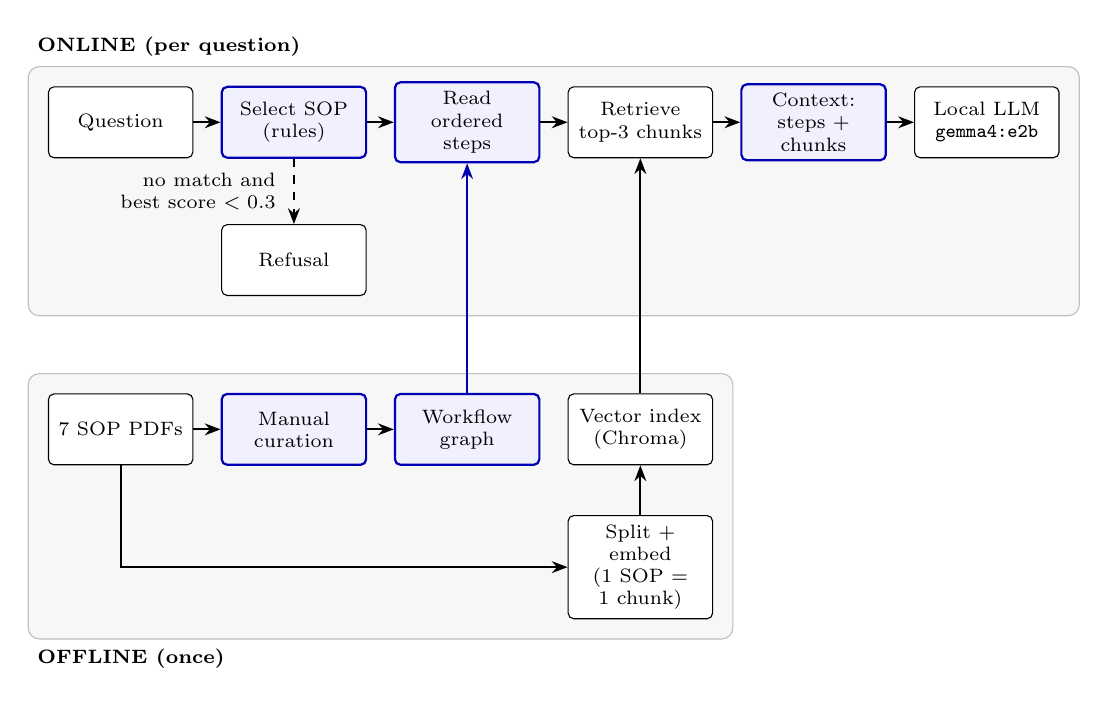
\begin{tikzpicture}[
  box/.style={draw, rounded corners=2pt, align=center, font=\scriptsize, minimum height=9mm, text width=16mm, fill=white},
  new/.style={box, draw=blue!70!black, fill=blue!6, thick},
  arr/.style={-{Stealth[length=2mm]}, thick},
  lane/.style={draw=gray!50, rounded corners=4pt, fill=gray!6, inner sep=2.5mm}
]
% Online row
\node[box] (q)    at (0,0)    {Question};
\node[new] (sel)  at (2.2,0)  {Select SOP\\(rules)};
\node[new] (read) at (4.4,0)  {Read ordered\\steps};
\node[box] (ret)  at (6.6,0)  {Retrieve\\top-3 chunks};
\node[new] (ctx)  at (8.8,0)  {Context:\\steps + chunks};
\node[box] (llm)  at (11.0,0) {Local LLM\\\texttt{gemma4:e2b}};
\node[box] (ref)  at (2.2,-1.75) {Refusal};
\draw[arr] (q) -- (sel);
\draw[arr] (sel) -- (read);
\draw[arr] (read) -- (ret);
\draw[arr] (ret) -- (ctx);
\draw[arr] (ctx) -- (llm);
\draw[arr, dashed] (sel) -- node[left, font=\scriptsize, align=right, xshift=-1mm]{no match and\\best score $<0.3$} (ref);
% Offline rows
\node[box] (pdf)    at (0,-3.9)   {7 SOP PDFs};
\node[new] (cur)    at (2.2,-3.9) {Manual\\curation};
\node[new] (graph)  at (4.4,-3.9) {Workflow\\graph};
\node[box] (chroma) at (6.6,-3.9) {Vector index\\(Chroma)};
\node[box] (split)  at (6.6,-5.65) {Split + embed\\(1 SOP = 1 chunk)};
\draw[arr] (pdf) -- (cur);
\draw[arr] (cur) -- (graph);
\draw[arr] (pdf.south) |- (split.west);
\draw[arr] (split) -- (chroma);
\draw[arr, blue!70!black] (graph) -- (read);
\draw[arr] (chroma) -- (ret);
\begin{scope}[on background layer]
\node[lane, fit=(q)(llm)(ref)] (on) {};
\node[lane, fit=(pdf)(split)(chroma)] (off) {};
\end{scope}
\node[font=\scriptsize\bfseries, anchor=south west] at (on.north west) {ONLINE (per question)};
\node[font=\scriptsize\bfseries, anchor=north west] at (off.south west) {OFFLINE (once)};
\end{tikzpicture}}
\caption{Architecture of Process-Aware Workflow GraphRAG. Highlighted nodes indicate components introduced: rule-based SOP selection and ordered workflow graph extraction. The underlying vector index, embedding model, prompt template, and generator are shared across evaluated systems.}
\label{fig:arch}
\end{figure}

\subsection{Workflow graph construction}
\label{sec:graph}
Each procedure $p$ is a directed graph $G_p=(V_p,E_p)$ implemented in NetworkX, with three node classes:
\begin{enumerate}[leftmargin=*]
\item \textbf{Root node ($v_{\text{root}}$):} the procedure, with its official title, aliases (e.g., ``cuti kuliah'' for academic leave), and maximum duration where stated.
\item \textbf{Step nodes ($v_i$), $i\in\{1,\dots,n_p\}$:} the performing actor, action, required input documents, outputs, duration, and a verbatim quote from the source PDF.
\item \textbf{Actor nodes ($v_{\text{actor}}$):} organisational roles shared across procedures.
\end{enumerate}
Edges are $\texttt{HAS\_STEP}(v_{\text{root}},v_i)$, $\texttt{NEXT\_STEP}(v_i,v_{i+1})$ for execution precedence, and $\texttt{PERFORMS}(v_{\text{actor}},v_i)$ for attribution. Built by hand from the 7 PDFs, the graph has 7 root, 44 step, and 15 actor nodes and 125 directed edges. A step's primary actor is the grammatical subject of its instruction; secondary signatories stay in the action description. Scripts verify that every quote matches the source verbatim and that step counts equal those of the PDFs. Figure~\ref{fig:graphs} contrasts this representation with the entity-graph baseline.

\begin{figure}[!htbp]
\centering
\resizebox{\textwidth}{!}{%
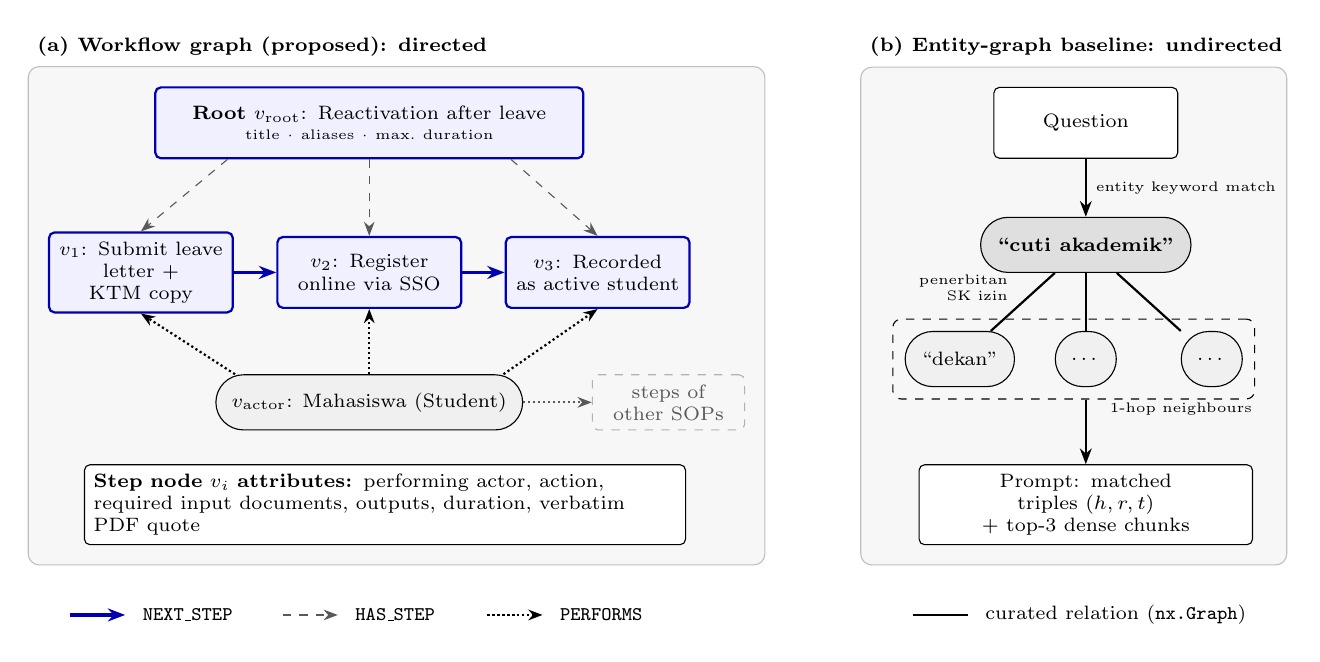
\begin{tikzpicture}[
  box/.style={execute at begin node={\hyphenpenalty=10000\exhyphenpenalty=10000}, draw, rounded corners=2pt, align=center, font=\scriptsize, minimum height=9mm, text width=21mm, fill=white},
  new/.style={box, draw=blue!70!black, fill=blue!6, thick},
  pill/.style={draw, rounded corners=3.5mm, align=center, font=\scriptsize, minimum height=7mm, inner xsep=2mm, fill=gray!12},
  ghost/.style={draw=gray!60, dashed, rounded corners=2pt, align=center, font=\scriptsize, text=gray!70!black, minimum height=7mm, text width=17mm},
  arr/.style={-{Stealth[length=2mm]}, thick},
  next/.style={-{Stealth[length=2.2mm]}, very thick, blue!70!black},
  has/.style={-{Stealth[length=1.8mm]}, gray!70!black, dashed},
  perf/.style={-{Stealth[length=1.8mm]}, densely dotted, thick},
  rel/.style={thick},
  lane/.style={draw=gray!50, rounded corners=4pt, fill=gray!6, inner sep=2.5mm}
]
% ===================== (a) Workflow graph (proposed) =====================
\node[new, text width=52mm] (root) at (2.9,0)
  {\textbf{Root} $v_{\text{root}}$: Reactivation after leave\\[-1pt]{\tiny title $\cdot$ aliases $\cdot$ max.\ duration}};
\node[new] (s1) at (0,-1.9)   {$v_1$: Submit leave\\letter + KTM copy};
\node[new] (s2) at (2.9,-1.9) {$v_2$: Register\\online via SSO};
\node[new] (s3) at (5.8,-1.9) {$v_3$: Recorded\\as active student};
\draw[has] (root.south) ++(-1.8,0) -- (s1.north);
\draw[has] (root.south) -- (s2.north);
\draw[has] (root.south) ++(1.8,0) -- (s3.north);
\draw[next] (s1) -- (s2);
\draw[next] (s2) -- (s3);
\node[pill] (act) at (2.9,-3.55) {$v_{\text{actor}}$: Mahasiswa (Student)};
\draw[perf] (act.north west) ++(0.25,0) -- (s1.south);
\draw[perf] (act.north) -- (s2.south);
\draw[perf] (act.north east) ++(-0.25,0) -- (s3.south);
\node[ghost] (oth) at (6.7,-3.55) {steps of\\other SOPs};
\draw[perf, gray!70!black] (act.east) -- (oth.west);
\node[draw, rounded corners=2pt, fill=white, font=\scriptsize, align=left, execute at begin node={\hyphenpenalty=10000}, text width=74mm] (attr) at (3.1,-4.85)
  {\textbf{Step node $v_i$ attributes:} performing actor, action, required input documents, outputs, duration, verbatim PDF quote};
% ===================== (b) Entity-graph baseline =====================
\node[box] (q) at (12.0,0) {Question};
\node[pill, fill=gray!25, font=\scriptsize\bfseries] (ent) at (12.0,-1.55) {``cuti akademik''};
\draw[arr] (q) -- node[right, font=\tiny]{entity keyword match} (ent);
\node[pill] (n1) at (10.4,-3.0)  {``dekan''};
\node[pill] (n2) at (12.0,-3.0) {\dots};
\node[pill] (n3) at (13.6,-3.0) {\dots};
\draw[rel] (ent) -- node[above left, pos=0.55, font=\tiny, align=right, inner sep=1pt, xshift=-1mm]{penerbitan\\SK izin} (n1);
\draw[rel] (ent) -- (n2);
\draw[rel] (ent) -- (n3);
\node[draw, dashed, rounded corners=3pt, fit=(n1)(n3), inner sep=1.5mm,
      label={[font=\tiny, anchor=north east, inner sep=1pt]south east:1-hop neighbours}] (hop) {};
\node[box, text width=40mm] (pr) at (12.0,-4.85) {Prompt: matched triples $(h,r,t)$\\+ top-3 dense chunks};
\draw[arr] (pr.north |- hop.south) -- (pr.north);
% ===================== Panels and legend =====================
\begin{scope}[on background layer]
\node[lane, fit=(root)(s1)(s3)(act)(oth)(attr)] (pa) {};
\node[lane, fit=(q)(n1)(n3)(hop)(pr), inner xsep=4mm] (pb) {};
\end{scope}
\node[font=\scriptsize\bfseries, anchor=south west] at (pa.north west) {(a) Workflow graph (proposed): directed};
\node[font=\scriptsize\bfseries, anchor=south west] at (pb.north west) {(b) Entity-graph baseline: undirected};
\begin{scope}[yshift=-6.25cm, font=\scriptsize]
\draw[next] (-0.9,0) -- (-0.2,0); \node[anchor=west] at (-0.1,0) {\texttt{NEXT\_STEP}};
\draw[has]  (1.8,0) -- (2.5,0);   \node[anchor=west] at (2.6,0)  {\texttt{HAS\_STEP}};
\draw[perf] (4.4,0) -- (5.1,0);   \node[anchor=west] at (5.2,0)  {\texttt{PERFORMS}};
\draw[rel]  (9.8,0) -- (10.5,0);   \node[anchor=west] at (10.6,0)  {curated relation (\texttt{nx.Graph})};
\end{scope}
\end{tikzpicture}}
\caption{Graph representations compared in this study. (a) The proposed directed workflow graph for the \emph{Reactivation after leave} SOP; the full graph has 7 root, 44 step, and 15 actor nodes and 125 edges. (b) The undirected entity-graph baseline: question entities are matched against 17 curated triples, and 1-hop triples are prepended to the top-3 dense chunks.}
\label{fig:graphs}
\end{figure}

\subsection{Rule-based SOP selection}
Given question $q$, the target procedure $p^\ast$ is identified with a transparent scoring function:
\begin{equation}
s(q,p) = 15\,\mathbb{1}[\textit{title}_p \subset q] + \sum_{a \in \textit{aliases}_p} g(q,a) + \sum_{v \in \textit{steps}_p} h(q,v),
\label{eq:score}
\end{equation}
where $g(q,a)=8$ if alias $a$ occurs as an exact substring of $q$, or 2 per constituent word ($|w|>2$); and $h(q,v)=1$ if $q$ contains an explicit procedural cue (Indonesian keywords for ``how'', ``procedure'', ``requirements'', ``flow'', or ``documents'') and shares a content word ($|w|>4$) with the action of step $v$. The highest-scoring procedure is selected if $s(q,p^\ast)\geq 3$. A priority rule sends questions with both ``active'' and ``leave'' keywords to \emph{Reactivation after leave}. The case-insensitive rules are inspectable but tailored to this collection.

\subsection{Context construction and supporting retrieval}
For the selected $p^\ast$, step nodes are traversed along \texttt{NEXT\_STEP} edges and serialized as an ordered block of step index, actor, action, documents, outputs, and duration (Figure~\ref{fig:context}).

\begin{figure}[!htbp]
\centering
\small
\fbox{\begin{minipage}{0.92\textwidth}
\textbf{OFFICIAL WORKFLOW: REACTIVATION AFTER LEAVE (AKTIF KEMBALI)}\\
Maximum processing duration: Not specified in document\\[2pt]
\textbf{Step 1.} Actor: Mahasiswa (Student)\\
\hspace*{1em}Action: Submit academic leave permit letter from prior semester and student card copy to Head of Study Programme and Academic Sub-division.\\
\hspace*{1em}Required Documents: Academic leave permit letter, Student card (KTM) copy\\
\hspace*{1em}Duration: $\pm$5 minutes\\[2pt]
\textbf{Step 2.} Actor: Mahasiswa (Student); Action: Register online through the SSO portal. \dots\\
\textbf{Step 3.} \dots\\[2pt]
\textbf{Supporting Documents:} \textit{[Top-3 dense chunks retrieved from vector store]}
\end{minipage}}
\caption{Context block produced for a reactivation question (translated from Indonesian).}
\label{fig:context}
\end{figure}

For supplementary details such as notes and URLs, the query is expanded with the SOP title and the actions of its first three steps, and $k=3$ chunks retrieved with it from the shared Chroma index are appended after the workflow block. Because each chunk is a whole SOP, these supporting chunks may contain other procedures, which we analyse in Section~\ref{sec:discussion}.

\subsection{Generation and refusal mechanism}
A standard template instructs \texttt{gemma4:e2b} (via Ollama) to answer in Indonesian from the provided facts only and to abstain when evidence is insufficient. Refusal is triggered deterministically before generation if (1) no SOP is selected ($s(q,p^\ast)<3$) and (2) the maximum cosine similarity between $q$ and the retrieved chunks is below $\tau=0.3$. Otherwise the generator may still abstain (Algorithm~\ref{alg:workflow}).

\begin{algorithm}[!htbp]
\caption{Execution pipeline of Process-Aware Workflow GraphRAG}
\label{alg:workflow}
\begin{algorithmic}[1]
\REQUIRE Question $q$, workflow graph $G$, vector index $I$, threshold $\tau = 0.3$, retrieval depth $k=3$
\STATE $p^\ast \leftarrow \arg\max_p s(q,p)$ \COMMENT{Evaluate selection via Eq.~\eqref{eq:score}}
\IF{$s(q,p^\ast) < 3$}
  \STATE $p^\ast \leftarrow \text{none}$
\ENDIF
\IF{$p^\ast \neq \text{none}$}
  \STATE $W \leftarrow$ serialized ordered step sequence of $p^\ast$ from $G$
  \STATE $q' \leftarrow q \,\|\, \textit{title}_{p^\ast} \,\|\, \textit{actions}_{1:3}(p^\ast)$ \COMMENT{Query expansion}
\ELSE
  \STATE $W \leftarrow \emptyset$
  \STATE $q' \leftarrow q$ \COMMENT{Retain unexpanded query}
\ENDIF
\STATE $C \leftarrow \textsc{RetrieveTopK}(I, q', k)$
\STATE $b \leftarrow \max_{c \in C} \textsc{CosineSimilarity}(q, c)$
\IF{$p^\ast = \text{none}$ \AND $b < \tau$}
  \RETURN Refusal response (``Information not available in official SOPs'')
\ENDIF
\RETURN $\textsc{GenerateLocalLLM}(\textsc{PromptTemplate}(W \,\|\, C, q))$
\end{algorithmic}
\end{algorithm}

\subsection{Selection-matched text ablation design}
\label{sec:ablation-oracle}
\emph{Selection-Matched Text RAG} (logged as \emph{SOP-Oracle RAG}) uses the same selection rule (Eq.~\eqref{eq:score}) and query-expanded supporting retrieval as Workflow GraphRAG but supplies the raw text chunk of $p^\ast$ instead of the serialized workflow $W$, so the two systems differ only in representation (Figure~\ref{fig:prompt}).

\begin{figure}[!htbp]
\centering
\resizebox{\textwidth}{!}{%
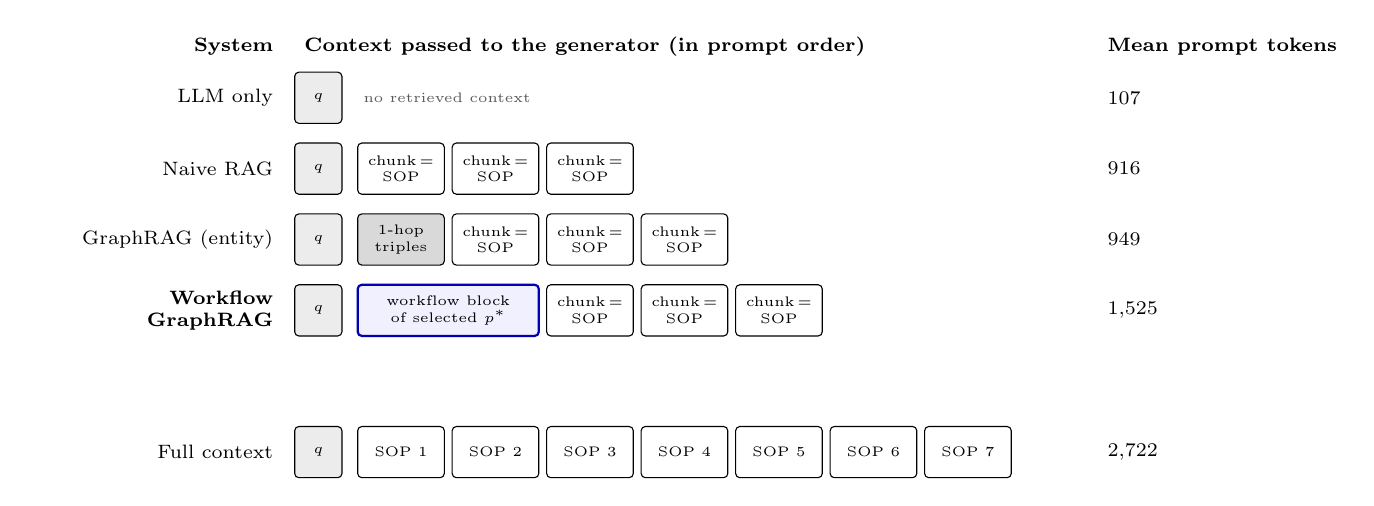
\begin{tikzpicture}[
  lab/.style={anchor=east, font=\scriptsize, align=right, text width=30mm},
  blk/.style={draw, rounded corners=1.5pt, font=\tiny, align=center, minimum height=6.5mm, minimum width=11mm, inner sep=1pt, fill=white},
  q/.style={blk, minimum width=6mm, fill=gray!15},
  sel/.style={blk, draw=blue!70!black, fill=blue!6, thick, minimum width=23mm},
  trip/.style={blk, fill=gray!30, minimum width=11mm},
  tok/.style={anchor=west, font=\scriptsize}
]
\def\dx{1.2}
% header
\node[font=\scriptsize\bfseries, anchor=east] at (-0.15,0.65) {System};
\node[font=\scriptsize\bfseries, anchor=west] at (0,0.65) {Context passed to the generator (in prompt order)};
\node[font=\scriptsize\bfseries, anchor=west] at (10.2,0.65) {Mean prompt tokens};
% LLM only
\node[lab] at (-0.15,0) {LLM only};
\node[q] at (0.3,0) {$q$};
\node[font=\tiny, anchor=west, text=gray!70!black] at (0.75,0) {no retrieved context};
\node[tok] at (10.2,0) {107};
% Naive
\node[lab] at (-0.15,-0.9) {Naive RAG};
\node[q] at (0.3,-0.9) {$q$};
\foreach \i in {1,2,3} \node[blk] at (0.75+\i*\dx-0.6,-0.9) {chunk\,=\\SOP};
\node[tok] at (10.2,-0.9) {916};
% Entity graph
\node[lab] at (-0.15,-1.8) {GraphRAG (entity)};
\node[q] at (0.3,-1.8) {$q$};
\node[trip] at (1.35,-1.8) {1-hop\\triples};
\foreach \i in {1,2,3} \node[blk] at (1.95+\i*\dx-0.6,-1.8) {chunk\,=\\SOP};
\node[tok] at (10.2,-1.8) {949};
% Workflow
\node[lab] at (-0.15,-2.7) {\textbf{Workflow GraphRAG}};
\node[q] at (0.3,-2.7) {$q$};
\node[sel] at (1.95,-2.7) {workflow block\\of selected $p^\ast$};
\foreach \i in {1,2,3} \node[blk] at (3.15+\i*\dx-0.6,-2.7) {chunk\,=\\SOP};
\node[tok] at (10.2,-2.7) {1,525};
% Selection-matched
\ifshoworacle
\node[lab] at (-0.15,-3.6) {Selection-Matched Text (ablation)};
\node[q] at (0.3,-3.6) {$q$};
\node[sel, thin, fill=blue!3] at (1.95,-3.6) {raw PDF text\\of selected $p^\ast$};
\foreach \i in {1,2,3} \node[blk] at (3.15+\i*\dx-0.6,-3.6) {chunk\,=\\SOP};
\node[tok] at (10.2,-3.6) {1,479};
\fi
% Full context
\node[lab] at (-0.15,-4.5) {Full context};
\node[q] at (0.3,-4.5) {$q$};
\foreach \i in {1,...,7} \node[blk] at (0.75+\i*\dx-0.6,-4.5) {SOP \i};
\node[tok] at (10.2,-4.5) {2,722};
\end{tikzpicture}}
\caption{Context supplied to the generator by the main comparison systems. Each chunk is a complete SOP, so top-3 retrieval always adds three procedures. Workflow GraphRAG and the ablation share selection and supporting chunks and differ only in how $p^\ast$ is represented. Token counts are means over all 40 questions, including the shared template.}
\label{fig:prompt}
\end{figure}

%% ===================================================================
\section{Experimental setup}
\label{sec:setup}

\subsection{Evaluated systems}
\label{sec:systems}
We evaluate 10 configurations in three groups (Table~\ref{tab:systems}): four main systems (Naive RAG, the custom entity-graph GraphRAG, Workflow GraphRAG, and the selection-matched ablation); four supplementary RAG baselines (Hybrid RAG \cite{robertson2009bm25,cormack2009rrf}, Agentic RAG \cite{yao2023react}, Corrective RAG \cite{yan2024crag}, and Multimodal-Layout RAG); and two reference systems (LLM only, which shows parametric knowledge without retrieval, and full-context prompting, which supplies all 7 SOPs as an upper bound on available evidence).

\begin{table}[!htbp]
\centering
\caption{System configurations evaluated across 10 architectures. All systems share identical embedding models, chunking parameters (1,700/100 characters), vector stores, generator, and prompt templates.}
\label{tab:systems}
\small
\begin{tabularx}{\textwidth}{>{\raggedright\arraybackslash}p{3.5cm} >{\raggedright\arraybackslash}X}
\toprule
System Configuration & Context Construction and Retrieval Mechanism \\
\midrule
\multicolumn{2}{l}{\textit{Main Comparison and Ablation}} \\
Naive RAG & Top-3 dense chunks by cosine similarity; refuses if best similarity $< 0.3$. \\
GraphRAG (custom entity graph) & 1-hop triples from 17 curated triples, prepended to top-3 dense chunks. \\
\textbf{Workflow GraphRAG (proposed)} & Ordered workflow block of the selected SOP, then top-3 supporting chunks. \\
\textit{Selection-Matched Text RAG (SOP-Oracle ablation)} & Same selection; raw text of the selected SOP instead of the workflow block, then top-3 supporting chunks. \\
\midrule
\multicolumn{2}{l}{\textit{Supplementary RAG Baselines}} \\
Hybrid RAG & Reciprocal rank fusion of top-5 dense and top-5 BM25 chunks ($k_{\text{rrf}}=60$); top-3 retained. \\
Agentic RAG & ReAct loop with up to 3 search actions. \\
Corrective RAG (CRAG) & Retrieval grading: $\geq 0.55$ retained, $0.35$--$0.55$ query rewritten, $< 0.35$ refused. \\
Multimodal-Layout RAG & Top-3 dense chunks with layout tags. \\
\midrule
\multicolumn{2}{l}{\textit{Reference Baselines}} \\
LLM Only & Zero-shot generation without retrieved context. \\
Full-Context Prompting & All 7 SOPs in the prompt ($\approx$1,100 words). \\
\bottomrule
\end{tabularx}
\end{table}

\subsection{Custom entity-graph baseline scope and validity threat}
The entity-graph baseline is our own implementation with 17 curated triples (Supplementary Material, S2), not Microsoft GraphRAG \cite{edge2024graphrag}, LightRAG \cite{guo2024lightrag}, or HippoRAG \cite{gutierrez2024hipporag}. It represents basic entity-triple augmentation rather than published GraphRAG frameworks (Section~\ref{sec:discussion}).

\subsection{Shared infrastructure and experimental controls}
All retrieval systems share the same infrastructure:
\begin{itemize}[leftmargin=*]
\item \textbf{Embedding model:} \texttt{all-indo-e5-small-v4} \cite{lazarusnlp_e5}, a 384-dimensional Indonesian E5-family \cite{wang2022e5} sentence embedder fine-tuned on 50 procedural question-answer pairs with Multiple Negatives Ranking loss \cite{henderson2017mnr}; an ablation uses the non-fine-tuned base model.
\item \textbf{Vector store:} Chroma, storing 7 chunks (1,700-character window, 100-character overlap).
\item \textbf{Generator:} \texttt{gemma4:e2b} (5.1B parameters, Q4\_K\_M quantization) served by Ollama 0.35.1 at temperature 0 and seed 42, after one warm-up inference.
\item \textbf{Hardware and logging:} an Apple M5 workstation (10 CPU cores, 24~GB unified memory) running macOS 26.6.2 on AC power; every generator call logs prompt tokens, completion tokens, and latency.
\end{itemize}

\subsection{Evaluation benchmark}
The held-out benchmark has 40 questions drafted from the SOPs (Table~\ref{tab:bench}): 35 answerable (32 single-SOP, 3 cross-SOP) and 5 unanswerable. No item was generated by an evaluated system, and none has ROUGE-L $\geq 0.5$ against the fine-tuning pairs. Answerable items define a reference answer and key facts; procedural items add gold steps, actors, and keyword groups. The first author verified all items against the PDFs; examples are given in the Supplementary Material (S3).

\begin{table}[!htbp]
\centering
\caption{Composition of the 40-question held-out institutional benchmark.}
\label{tab:bench}
\small
\setlength{\tabcolsep}{4pt}
\begin{tabularx}{\textwidth}{lr>{\raggedright\arraybackslash}X}
\toprule
Category & $n$ & Operational Target \\
\midrule
Procedural & 11 & Complete step sequence, chronological order, and actors (7 formal, 4 colloquial). \\
Actor attribution & 7 & Identification of verifying, signing, or receiving officials. \\
Document requirements & 7 & Identification of mandatory forms, attachments, and outputs. \\
Time and location & 7 & Stated execution durations, service desks, and IT portals. \\
Cross-SOP discrimination & 3 & Differentiating easily confused procedures (evaluating E3). \\
Unanswerable / Refusal & 5 & Inquiries concerning out-of-scope administrative rules. \\
\midrule
Total & 40 & \\
\bottomrule
\end{tabularx}
\end{table}

\subsection{Evaluation metrics}
All primary metrics are computed deterministically, without LLM judges:
\begin{itemize}[leftmargin=*]
\item \textbf{Key-Fact Recall (KFR):} share of required key facts found in the response (35 answerable questions).
\item \textbf{ROUGE-1/2/L:} overlap with the reference answer \cite{lin2004rouge}.
\item \textbf{Step Coverage:} share of gold steps $S$ detected ($|D|/|S|$) on the 11 procedural questions; detection requires two matching keyword groups.
\item \textbf{Topological Inversion Rate (TIR):} share of detected step pairs $(v_i,v_j)$ with $i<j$ that appear in reversed order:
\begin{equation}
\text{TIR} = \frac{\bigl|\{(v_i,v_j) \in D^2 : i<j,\ \textit{pos}(v_i) > \textit{pos}(v_j)\}\bigr|}{\bigl|\{(v_i,v_j) \in D^2 : i<j,\ \textit{pos}(v_i) \neq \textit{pos}(v_j)\}\bigr|},
\end{equation}
defined only when at least two comparable steps are detected.
\item \textbf{Actor Mismatch Rate (AMR):} among detected steps with an explicitly named actor, the share attributed to the wrong official:
\begin{equation}
\text{AMR} = \frac{\textit{mismatch}}{\textit{correct} + \textit{mismatch}}.
\end{equation}
\item \textbf{Refusal accuracy / false refusal rate:} share of the 5 unanswerable questions refused / of the 35 answerable questions refused.
\item \textbf{Resource costs:} tokens, LLM calls, and latency per question (all 40 items).
\end{itemize}

\subsection{Manual audit of deterministic step scorer}
\label{sec:audit}
Because step detection, TIR, and AMR rely on keyword matching, the first author checked 60 step-alignment rows, sampled across Naive RAG, GraphRAG, and Workflow GraphRAG (stratified, seed 42), against the full response texts (Table~\ref{tab:audit}).

\begin{table}[!htbp]
\centering
\caption{Manual audit of deterministic step-alignment scorer across 60 sampled rows (Naive RAG, GraphRAG, and Workflow GraphRAG).}
\label{tab:audit}
\small
\begin{tabular}{lcc}
\toprule
Measure & Agreement / $\kappa$ & Labelled \\
\midrule
Step detected & 0.983 / 0.955 & 60/60 \\
Actor status & 0.933 / 0.835 & 60/60 \\
\bottomrule
\end{tabular}

\end{table}

Agreement was 0.983 ($\kappa=0.955$) for step detection and 0.933 ($\kappa=0.835$) for actor attribution. The one detection miss (GraphRAG, UKT-P1, step 5) occurred because actor and action sat on separate markdown lines, while the scorer needs two keyword groups on one line. No genuine actor error was found in the sample ($\text{AMR}=0.000$).

\subsection{Secondary LLM-as-a-judge metrics}
Ragas faithfulness and answer relevancy \cite{es2024ragas}, judged by \texttt{llama3.1:8b} \cite{zheng2023judging}, serve only as secondary evidence, because judge parsing failures leave valid scores for 35/40 questions (Workflow GraphRAG) and 26--27/40 (baselines).

\subsection{Statistical testing methodology}
Metrics are means with 95\% bootstrap intervals (10,000 resamples) \cite{efron1993bootstrap}. Workflow GraphRAG is compared with baselines by two-sided paired Wilcoxon signed-rank tests \cite{wilcoxon1945} with Holm-Bonferroni correction \cite{holm1979} within each family (versus Naive RAG and versus GraphRAG). An unadjusted interval can exclude zero while the adjusted $p$ exceeds 0.05; we report both and never read non-significance as equivalence.

%% ===================================================================
\section{Experimental results}
\label{sec:results}

All results come from the run on the \nVerified{} verified benchmark items (\url{results/full_v3_20261008/}, branch \url{exp/full-run-v1}).

\subsection{Procedural answer quality and order preservation (RQ1)}
Table~\ref{tab:results} reports all 10 systems. Workflow GraphRAG, Selection-Matched Text RAG, and full-context prompting reach the highest key-fact recall (0.955, 0.962, and 0.962), against 0.712 for Naive RAG and 0.698 for the entity-graph baseline; Workflow GraphRAG also reaches 1.000 step coverage (0.727 and 0.687). Confidence intervals are given in the Supplementary Material (S1).

\begin{table}[!htbp]
\centering
\caption{Summary of evaluation results across ten system configurations. KFR and false refusal: 35 answerable questions; Coverage, TIR, and AMR: 11 procedural questions; refusal accuracy: 5 unanswerable questions; prompt tokens: all 40. Point estimates; confidence intervals are in the Supplementary Material (S1).}
\label{tab:results}
\small
\setlength{\tabcolsep}{2pt}
\resizebox{\textwidth}{!}{%
\begin{tabular}{lccccccc}
\toprule
System & KFR $\uparrow$ & Coverage $\uparrow$ & TIR $\downarrow$ & AMR $\downarrow$ & Refusal acc. $\uparrow$ & False ref. $\downarrow$ & Prompt tok. \\
\midrule
Naive RAG & 0.712 & 0.727 & 0.000 & 0.000 & 0.600 & 0.000 & 916 \\
GraphRAG (entity) & 0.698 & 0.687 & 0.083 & 0.000 & 0.600 & 0.000 & 949 \\
\textbf{Workflow GraphRAG} & 0.955 & 1.000 & 0.000 & 0.000 & 1.000 & 0.000 & 1525 \\
\textit{Selection-Matched Text RAG (ablation)} & 0.962 & 0.975 & 0.000 & 0.000 & 1.000 & 0.000 & 1479 \\
\midrule
Hybrid RAG & 0.683 & 0.712 & 0.000 & 0.000 & 0.600 & 0.000 & 882 \\
Agentic RAG & 0.712 & 0.702 & 0.000 & 0.000 & 0.600 & 0.000 & 1815 \\
Corrective RAG & 0.569 & 0.636 & 0.000 & 0.000 & 1.000 & 0.371 & 725 \\
Multimodal-layout RAG & 0.702 & 0.702 & 0.000 & 0.000 & 0.600 & 0.000 & 994 \\
\midrule
LLM only & 0.113 & 0.105 & 0.333 & 0.444 & 0.000 & 0.000 & 107 \\
Full context & 0.962 & 0.944 & 0.027 & 0.000 & 1.000 & 0.000 & 2722 \\
\bottomrule
\end{tabular}
}
\end{table}

Against GraphRAG, Workflow GraphRAG improves key-fact recall by $+0.257$ [0.133, 0.395] (Holm-adjusted $p=0.034$) and ROUGE-L by $+0.077$ [0.031, 0.127] (Holm-adjusted $p=0.038$); the step-coverage difference is not significant after adjustment ($p=0.438$). Against Naive RAG, the recall gain of $+0.243$ [0.114, 0.381] has a Holm-adjusted $p=0.053$ and therefore does not reach significance at $\alpha=0.05$, although the unadjusted interval excludes zero; with $n=40$, statistical power is limited.

On detected steps, TIR is 0.000 for Workflow GraphRAG, Naive RAG, Selection-Matched Text RAG, and the supplementary baselines, but 0.083 for the entity-graph baseline, 0.027 for full-context prompting, and 0.333 for LLM only; AMR is 0.000 for every retrieval-augmented system and 0.444 for LLM only. Both metrics are conditional on detection, so systems differ mainly in completeness rather than in reordering.

By category (Table~\ref{tab:percat}), Workflow GraphRAG reaches 1.000 key-fact recall on procedural questions (0.727 for both baselines) and 0.889 on cross-SOP questions (0.611). Explicit step outputs let it attribute signatories across procedures, mitigating E3.

\begin{table}[!htbp]
\centering
\caption{Key-fact recall by question category for the primary comparison systems on \nVerified{} verified questions. Procedural category also includes step coverage.}
\label{tab:percat}
\small
\setlength{\tabcolsep}{4pt}
\resizebox{\textwidth}{!}{%
% Key-fact recall per category (procedural column also has step coverage), for the three main systems
\begin{tabular}{lccccc}
\toprule
System & Procedural (KFR/Cov.) & Actor & Documents & Time/location & Cross-SOP \\
\midrule
Naive RAG & 0.727 / 0.727 & 0.857 & 0.619 & 0.679 & 0.611 \\
GraphRAG (entity) & 0.727 / 0.687 & 0.786 & 0.619 & 0.679 & 0.611 \\
\textbf{Workflow GraphRAG} & 1.000 / 1.000 & 0.952 & 0.905 & 0.964 & 0.889 \\
\bottomrule
\end{tabular}
}
\end{table}

\subsection{Selection versus structuring ablation (RQ2)}
\label{sec:ablation-results}
Workflow GraphRAG (0.955 KFR) and Selection-Matched Text RAG (0.962 KFR) differ only in whether the selected procedure arrives as a workflow block or as raw PDF text. On the 35 answerable questions the paired difference is $-0.007$ [$-0.036$, $0.021$] (Wilcoxon $p=0.59$), and scores differ on only 3 questions (Figure~\ref{fig:forest}). This is not proof of equivalence, but the data show no evidence that graph serialization adds factual accuracy over the selected raw text.

\begin{figure}[!htbp]
\centering
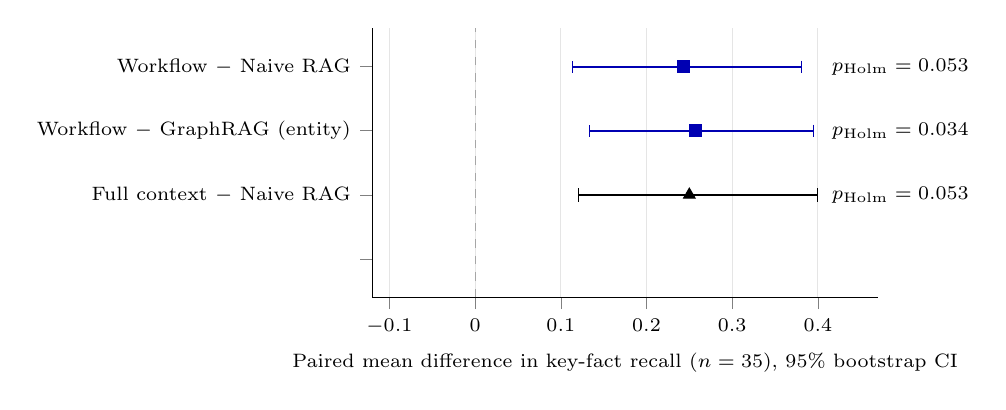
\begin{tikzpicture}
\begin{axis}[
  width=0.66\textwidth, height=5.0cm,
  xmin=-0.12, xmax=0.47, ymin=0.4, ymax=4.6,
  ytick={1,2,3,4},
  yticklabels={
    \ifshoworacle Workflow $-$ Selection-Matched\else\fi,
    Full context $-$ Naive RAG,
    Workflow $-$ GraphRAG (entity),
    Workflow $-$ Naive RAG},
  yticklabel style={font=\scriptsize, align=right},
  xticklabel style={font=\scriptsize, /pgf/number format/fixed, /pgf/number format/precision=2},
  xlabel={Paired mean difference in key-fact recall ($n=35$), 95\% bootstrap CI},
  xlabel style={font=\scriptsize},
  axis lines*=left, tick align=outside, clip=false,
  xmajorgrids, grid style={gray!20},
]
\draw[gray!70, dashed] (axis cs:0,0.4) -- (axis cs:0,4.6);
% Workflow - Naive: 0.243 [0.114, 0.381], Holm p = 0.053
\addplot[blue!70!black, only marks, mark=square*, mark size=2.2pt, error bars/.cd, x dir=both, x explicit, error bar style={thick}]
  coordinates {(0.243,4) += (0.138,0) -= (0.129,0)};
% Workflow - GraphRAG: 0.257 [0.133, 0.395], Holm p = 0.034
\addplot[blue!70!black, only marks, mark=square*, mark size=2.2pt, error bars/.cd, x dir=both, x explicit, error bar style={thick}]
  coordinates {(0.257,3) += (0.138,0) -= (0.124,0)};
% Full context - Naive: 0.250 [0.121, 0.400], Holm p = 0.053
\addplot[black, only marks, mark=triangle*, mark size=2.4pt, error bars/.cd, x dir=both, x explicit, error bar style={thick}]
  coordinates {(0.250,2) += (0.150,0) -= (0.129,0)};
\ifshoworacle
% Workflow - Selection-Matched: -0.007 [-0.036, 0.021], Wilcoxon p = 0.59 (paper text; not in repository)
\addplot[blue!70!black, only marks, mark=square, mark size=2.2pt, error bars/.cd, x dir=both, x explicit, error bar style={thick}]
  coordinates {(-0.007,1) += (0.028,0) -= (0.029,0)};
\node[font=\scriptsize, anchor=west] at (axis cs:0.405,1) {$p=0.59$};
\fi
\node[font=\scriptsize, anchor=west] at (axis cs:0.405,4) {$p_{\mathrm{Holm}}=0.053$};
\node[font=\scriptsize, anchor=west] at (axis cs:0.405,3) {$p_{\mathrm{Holm}}=0.034$};
\node[font=\scriptsize, anchor=west] at (axis cs:0.405,2) {$p_{\mathrm{Holm}}=0.053$};
\end{axis}
\end{tikzpicture}
\caption{Paired differences in key-fact recall on the 35 answerable questions, with 95\% bootstrap intervals and Wilcoxon $p$-values (Holm-adjusted within each reference family). With selection held fixed, the difference is near zero.}
\label{fig:forest}
\end{figure}

The step-coverage gap (1.000 vs.\ 0.975) comes from one item (UKT-P1), where the ablation split actors and actions across lines and the scorer missed steps that were present (Section~\ref{sec:audit}).

The selector routed all 32 answerable single-SOP questions correctly and misrouted none (Table~\ref{tab:selection}); for each cross-SOP question it chose one of the procedures involved. Ragas scores agree: faithfulness/relevancy are 0.805/0.682 for Workflow GraphRAG, 0.762/0.549 for Naive RAG, and 0.743/0.537 for GraphRAG.

\begin{table}[!htbp]
\centering
\caption{Outcome of the rule-based SOP selector (Eq.~\eqref{eq:score}) for Workflow GraphRAG on all 40 benchmark questions, read from the \texttt{matched\_sop} field of the run log.}
\label{tab:selection}
\small
\setlength{\tabcolsep}{4pt}
\begin{tabularx}{\textwidth}{>{\raggedright\arraybackslash}p{2.7cm} r >{\raggedright\arraybackslash}X >{\raggedright\arraybackslash}p{3.0cm}}
\toprule
Question group & $n$ & Selector outcome & Consequence \\
\midrule
Answerable, single SOP & 32 & Correct SOP selected (32/32) & Workflow block of correct SOP in prompt \\
Answerable, cross-SOP (X-1--X-3) & 3 & One of the involved SOPs selected (X-1: Reactivation; X-2: Academic leave; X-3: Course registration) & Other SOPs reach the prompt only via supporting chunks \\
Unanswerable, SOP topic (NA-1--NA-3) & 3 & Topical SOP selected & Generator abstained (3/3) \\
Unanswerable, no match (NA-4, NA-5) & 2 & No SOP reaches $s \geq 3$ & Deterministic refusal before generation \\
\midrule
Total & 40 & No misrouting between procedures & \\
\bottomrule
\end{tabularx}
\end{table}

\subsection{Refusal and boundary handling (RQ3)}
Workflow GraphRAG, Selection-Matched Text RAG, and full-context prompting refuse all 5 unanswerable questions with no false refusals (Table~\ref{tab:results}). LLM only never abstains (0.000 refusal accuracy; the 0.333 in earlier drafts was a column transposition of its TIR), and Corrective RAG also refuses 13 of 35 answerable questions (false refusal rate 0.371) because of its threshold ($\tau=0.35$).

The 0.600 refusal accuracy of Naive RAG, GraphRAG, Hybrid, Agentic, and Multimodal-Layout RAG is partly a scoring artefact. Below $\tau=0.30$, Naive RAG returns a fixed template (``\textit{Maaf, saya tidak menemukan jawaban pada dokumen SOP resmi yang tersedia}'') without calling the generator, on 10 queries (8 answerable, plus NA-4 and NA-5). Because the refusal patterns omitted ``\textit{tidak menemukan}'', the template was scored as a non-refusal: the 8 answerable queries received $\text{KFR}=0.000$ without counting as false refusals, and NA-4 and NA-5 counted as failed refusals; only NA-1 to NA-3 (``\textit{tidak ditemukan}'') were credited.

Workflow GraphRAG refused NA-4 and NA-5 before inference (no SOP scored 3; similarity below 0.3). For NA-1 to NA-3 a topical SOP was selected and the generator stated that the requested fee or GPA criteria are not in the SOP, so questions that mention SOP keywords still reach the generator: an operational boundary, not a general check of evidence sufficiency.

\subsection{Computational efficiency and resource trade-offs (RQ4)}
Workflow GraphRAG uses 1,525 prompt tokens per query (Table~\ref{tab:cost}), more than Naive RAG (916) and GraphRAG (949) because of the workflow block, but 44\% fewer than full-context prompting (2,722) at close recall (0.955 vs.\ 0.962; Figure~\ref{fig:tradeoff}).

\begin{figure}[!htbp]
\centering
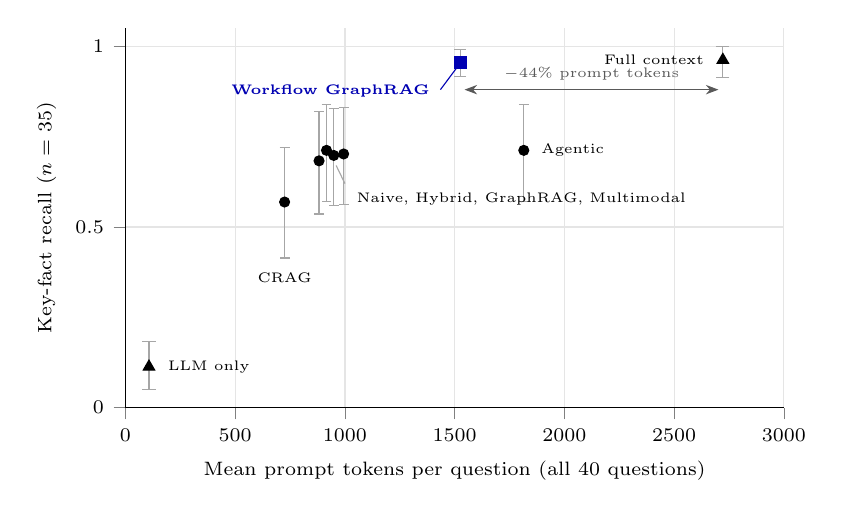
\begin{tikzpicture}
\begin{axis}[
  width=0.82\textwidth, height=6.4cm,
  xmin=0, xmax=3000, ymin=0, ymax=1.05,
  xlabel={Mean prompt tokens per question (all 40 questions)},
  ylabel={Key-fact recall ($n=35$)},
  xlabel style={font=\scriptsize}, ylabel style={font=\scriptsize},
  ticklabel style={font=\scriptsize},
  scaled x ticks=false, xtick={0,500,...,3000}, xticklabel style={/pgf/number format/1000 sep={}},
  axis lines*=left, tick align=outside, clip=false,
  grid=major, grid style={gray!20},
  error bars/error bar style={gray!70},
]
% chunk-retrieval baselines
\addplot[black, only marks, mark=*, mark size=1.8pt, error bars/.cd, y dir=both, y explicit]
coordinates {
 (916,0.712)  += (0,0.128) -= (0,0.141)
 (882,0.683)  += (0,0.136) -= (0,0.147)
 (949,0.698)  += (0,0.131) -= (0,0.138)
 (994,0.702)  += (0,0.129) -= (0,0.140)
 (1815,0.712) += (0,0.128) -= (0,0.141)
 (725,0.569)  += (0,0.150) -= (0,0.155)
};
% reference systems
\addplot[black, only marks, mark=triangle*, mark size=2.4pt, error bars/.cd, y dir=both, y explicit]
coordinates {
 (107,0.113)  += (0,0.070) -= (0,0.063)
 (2722,0.962) += (0,0.038) -= (0,0.048)
};
% proposed
\addplot[blue!70!black, only marks, mark=square*, mark size=2.2pt, error bars/.cd, y dir=both, y explicit]
coordinates {(1525,0.955) += (0,0.035) -= (0,0.038)};
\ifshoworacle
\addplot[blue!70!black, only marks, mark=square, mark size=2.2pt, error bars/.cd, y dir=both, y explicit]
coordinates {(1479,0.962) += (0,0.038) -= (0,0.048)};
\node[font=\tiny, anchor=east, blue!70!black] at (axis cs:1440,1.01) {Selection-Matched};
\fi
% labels
\node[font=\tiny, anchor=north west] at (axis cs:1010,0.62) {Naive, Hybrid, GraphRAG, Multimodal};
\draw[gray!70, thin] (axis cs:1000,0.62) -- (axis cs:960,0.67);
\node[font=\tiny, anchor=north] at (axis cs:725,0.40) {CRAG};
\node[font=\tiny, anchor=west] at (axis cs:1850,0.712) {Agentic};
\node[font=\tiny, anchor=west] at (axis cs:150,0.113) {LLM only};
\node[font=\tiny, anchor=east, blue!70!black] at (axis cs:1430,0.875) {\textbf{Workflow GraphRAG}};
\draw[blue!70!black, thin] (axis cs:1435,0.88) -- (axis cs:1515,0.945);
\node[font=\tiny, anchor=east] at (axis cs:2680,0.962) {Full context};
\draw[{Stealth[length=1.6mm]}-{Stealth[length=1.6mm]}, gray!70!black] (axis cs:1545,0.88) -- node[above, font=\tiny]{$-44\%$ prompt tokens} (axis cs:2702,0.88);
\end{axis}
\end{tikzpicture}
\caption{Key-fact recall against mean prompt tokens for all evaluated systems. Error bars: 95\% bootstrap intervals. Circles: chunk-retrieval baselines; triangles: reference systems; squares: systems with rule-based SOP selection.}
\label{fig:tradeoff}
\end{figure}

\begin{table}[!htbp]
\centering
\caption{Operational resource consumption per query across evaluated systems: mean prompt and completion tokens, mean generator invocations, and median execution latency across all 40 questions.}
\label{tab:cost}
\small
\setlength{\tabcolsep}{4pt}
\resizebox{\textwidth}{!}{%
\begin{tabular}{lcccc}
\toprule
System & Prompt tok. & Completion tok. & LLM calls & Latency (s) \\
\midrule
Naive RAG & 916 & 555 & 0.75 & 9.9 \\
GraphRAG (entity) & 949 & 559 & 0.75 & 9.6 \\
\textbf{Workflow GraphRAG} & 1525 & 710 & 0.95 & 10.7 \\
Hybrid RAG & 882 & 566 & 0.75 & 9.3 \\
Agentic RAG & 1815 & 1857 & 3.27 & 28.7 \\
Corrective RAG & 725 & 661 & 1.05 & 12.7 \\
Multimodal-layout RAG & 994 & 561 & 0.75 & 9.8 \\
LLM only & 107 & 792 & 1.00 & 10.4 \\
Full context & 2722 & 792 & 1.00 & 12.1 \\
\bottomrule
\end{tabular}
}
\end{table}

Calls per query reflect pre-generation refusal ($30/40=0.75$ for chunk baselines, $38/40=0.95$ for Workflow GraphRAG, 1.00 for full context), whereas Agentic RAG averages 3.27 calls, 1,815 prompt tokens, and 28.7~s median latency without better recall (0.712 KFR). Workflow GraphRAG's median latency is 10.7~s (Naive RAG 9.9~s; full context 12.1~s); hardware cost was not priced.

\subsection{Embedding sensitivity ablation}
\label{sec:ablation-embedding}
With the non-fine-tuned base \texttt{all-indo-e5-small-v4} model (Figure~\ref{fig:embedding}), Naive RAG rises from 0.712 to 0.910 KFR (step coverage 0.727 to 0.898) and GraphRAG from 0.698 to 0.900, while Workflow GraphRAG stays at 0.955. Overfitting to the 50 fine-tuning pairs is plausible but untested against alternatives such as objective mismatch or training instability. Either way, well-configured chunk retrieval is competitive on this corpus, which narrows the margin for workflow-guided retrieval.

\begin{figure}[!htbp]
\centering
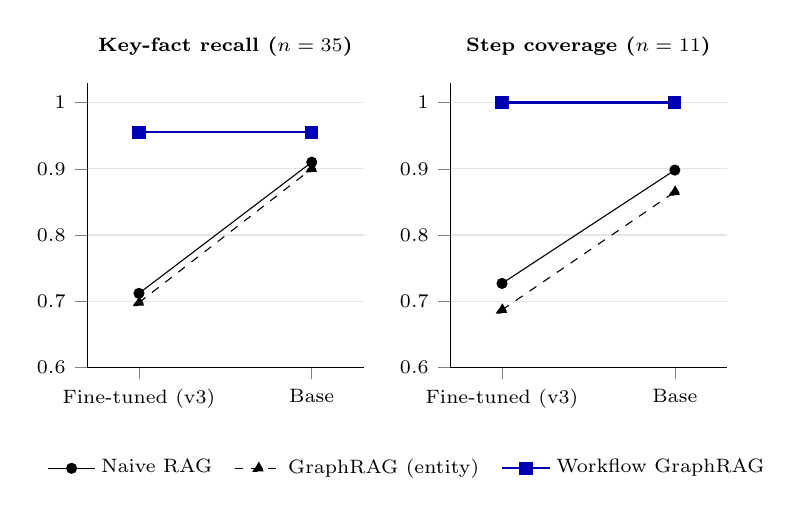
\begin{tikzpicture}
\pgfplotsset{abl/.style={
  width=0.42\textwidth, height=5.2cm,
  xmin=-0.3, xmax=1.3, ymin=0.6, ymax=1.03,
  xtick={0,1}, xticklabels={Fine-tuned (v3), Base},
  ticklabel style={font=\scriptsize}, title style={font=\scriptsize\bfseries},
  axis lines*=left, tick align=outside, ymajorgrids, grid style={gray!20},
  yticklabel style={/pgf/number format/fixed, /pgf/number format/precision=2}}}
\begin{axis}[abl, name=kfr, title={Key-fact recall ($n=35$)}]
\addplot[black, mark=*, mark size=1.8pt] coordinates {(0,0.712) (1,0.910)};
\addplot[black, dashed, mark=triangle*, mark size=2.2pt] coordinates {(0,0.698) (1,0.900)};
\addplot[blue!70!black, thick, mark=square*, mark size=2pt] coordinates {(0,0.955) (1,0.955)};
\end{axis}
\begin{axis}[abl, at={(kfr.east)}, anchor=west, xshift=1.1cm, title={Step coverage ($n=11$)},
  legend style={font=\scriptsize, draw=none, at={(-0.15,-0.28)}, anchor=north, legend columns=3, /tikz/every even column/.append style={column sep=6pt}}]
\addplot[black, mark=*, mark size=1.8pt] coordinates {(0,0.727) (1,0.898)};
\addplot[black, dashed, mark=triangle*, mark size=2.2pt] coordinates {(0,0.687) (1,0.865)};
\addplot[blue!70!black, thick, mark=square*, mark size=2pt] coordinates {(0,1.000) (1,1.000)};
\legend{Naive RAG, GraphRAG (entity), Workflow GraphRAG}
\end{axis}
\end{tikzpicture}
\caption{Embedding sensitivity: key-fact recall and step coverage with the fine-tuned (v3) and the non-fine-tuned base \texttt{all-indo-e5-small-v4} embedding. Chunk-retrieval baselines improve markedly with the base model, whereas Workflow GraphRAG is unchanged.}
\label{fig:embedding}
\end{figure}

\subsection{Qualitative error analysis}
In the cross-SOP question X-2 (``Who signs the academic leave permit and late tuition permit letters, respectively?''), Naive RAG retrieved both procedures but listed several candidate signatories under each (KFR = 0.5), whereas Workflow GraphRAG used step outputs to answer ``Dean for Academic Leave Permit; Vice Dean for Resources for Late Tuition Permit'' (KFR = 1.0). For IRS-A1 (``Who approves the IRS form and how?''), it named the academic advisor and the SIAP portal but omitted that approval follows credit-load verification (KFR = 0.667).

%% ===================================================================
\section{Discussion and threats to validity}
\label{sec:discussion}

\subsection{Empirical findings and architectural interpretation}
The results support two conclusions. First, the complete pipeline reaches high completeness (0.955 KFR, 1.000 step coverage) with 44\% fewer prompt tokens than full-context prompting. Second, graph serialization was \emph{not} shown to add factual accuracy over the selected raw text ($p=0.59$).

In concise, linear workflows, procedure-level selection is thus the key differentiator from unconstrained retrieval, which injects three competing procedures; routing rules, metadata filters, or workflow indexes can all provide it, although our design does not fully separate selection from the accompanying query expansion and context budget. The value of explicit structure lies in consistent formatting, compact prompts, and explicit deliverable attribution rather than in higher recall.

\subsection{Threats to internal and comparative validity}
\begin{itemize}[leftmargin=*]
\item \textbf{Custom baseline:} the 17-triple entity-graph baseline is not an automated framework such as Microsoft GraphRAG \cite{edge2024graphrag} or LightRAG \cite{guo2024lightrag}; $p=0.034$ holds against this baseline only.
\item \textbf{Benchmark curation:} items were written and verified by the first author, not an independent administrative panel.
\item \textbf{Sample size:} with 40 questions, power is limited, as the borderline comparison with Naive RAG ($p=0.053$) shows.
\item \textbf{Audit scope:} 60 sampled rows from three systems support scorer reliability but cannot rule out actor errors in uninspected outputs.
\end{itemize}

\subsection{Corpus and generalizability limitations}
\begin{itemize}[leftmargin=*]
\item \textbf{Short linear procedures:} 7 one-page procedures (1,097 words) without branching or gateways; results may not transfer to branching enterprise workflows.
\item \textbf{Selector transferability:} the alias rules suit 7 SOPs; hundreds of procedures would need learned classification or hierarchical routing.
\item \textbf{Supporting-chunk contamination:} appended top-3 chunks reintroduce unselected SOPs; restricting them to the selected SOP should be tested.
\item \textbf{Single generator:} only \texttt{gemma4:e2b} at temperature 0 was tested; other families (e.g., Llama-3.2, Qwen-2.5) are needed.
\end{itemize}

%% ===================================================================
\section{Conclusion and future work}
\label{sec:conclusion}

Across 10 configurations and 40 verified questions with \texttt{gemma4:e2b}, Workflow GraphRAG reached 0.955 KFR and 1.000 step coverage with an observed TIR of 0.000 (RQ1), the selection-matched ablation matched it at 0.962 KFR ($p=0.59$; RQ2), all unanswerable questions were refused (RQ3), and the workflow block used 44\% fewer prompt tokens than full-context prompting (RQ4).

For small models over concise procedures, procedure-level selection is the main lever against cross-document distractors; workflow graphs add ordered output and shorter prompts but no extra recall over well-selected raw text. Future work will learn the selector, parse branching procedures from BPMN XML, compare with LightRAG and HippoRAG, and run an a priori powered evaluation with independent administrative validation.

\section*{Acknowledgements}
This research did not receive any specific grant from funding agencies in the public, commercial, or not-for-profit sectors. The authors thank the Dean of the Faculty of Science and Mathematics, Universitas Diponegoro, Prof.\ Dr.\ Kusworo Adi, the Head of the Department of Informatics, Dr.\ Aris Sugiharto, the Undergraduate Thesis Coordinator, Nurdin Bahtiar, and the thesis examiners, Dr.\ Sutikno and Yunila Dwi Putri Ariyanti, for their guidance and feedback, and the Faculty of Science and Mathematics for permitting this research to be carried out using its SOPs.

\section*{Data and code availability}
Code, benchmark, and evaluation scripts are available at \url{https://github.com/reon01425-glitch/Chatbot-RAG-Comparison}, branch \url{exp/full-run-v1}. Experimental logs are deposited in \url{results/full_v3_20261008/} (main run) and \url{results/full_base_20261008/} (embedding ablation). The repository includes the 7 source SOP documents redistributed under institutional permission.

\section*{CRediT authorship contribution statement}
\textbf{Cipta Fikri Wiratama}: Conceptualization, Methodology, Software, Data curation, Validation, Investigation, Writing -- original draft. \textbf{Indra Waspada}: Conceptualization, Supervision, Writing -- review \& editing. \textbf{Dhena Kamalia Fu'adi}: Data curation, Validation, Writing -- review \& editing. \textbf{Ramona Ramli}: Conceptualization, Methodology, Supervision, Writing -- review \& editing. \textbf{Henri Tantyoko}: Methodology, Validation, Writing -- review \& editing. \textbf{Sandy Kurniawan}: Supervision, Methodology, Writing -- review \& editing. \textbf{Satriawan Rasyid Purnama}: Validation, Formal analysis, Writing -- review \& editing.

\section*{Ethics statement}
This study did not involve human participants, personal data, or animals. The benchmark questions and reference answers were written by the authors, and the SOP documents were used with the permission of the Faculty of Science and Mathematics, Universitas Diponegoro.

\section*{Declaration of competing interest}
The authors declare no competing interests.

\section*{Declaration of generative AI use}
During the preparation of this work, the authors used generative AI tools to assist with productivity in literature search, drafting, and academic language editing. All methodological formulations, system implementations, and experimental analyses were designed by the authors, who reviewed and edited all generated text and assume full responsibility for the published content.

\small
\setlength{\bibsep}{2pt}
\begin{thebibliography}{99}

\bibitem{lewis2020rag}
P.~Lewis, E.~Perez, A.~Piktus, F.~Petroni, V.~Karpukhin, N.~Goyal, H.~K{\"u}ttler, M.~Lewis, W.~Yih, T.~Rockt{\"a}schel, S.~Riedel, D.~Kiela, Retrieval-augmented generation for knowledge-intensive {NLP} tasks, in: Advances in Neural Information Processing Systems 33 (NeurIPS 2020), 2020, pp. 9459--9474.

\bibitem{gao2023ragsurvey}
Y.~Gao, Y.~Xiong, X.~Gao, K.~Jia, J.~Pan, Y.~Bi, Y.~Dai, J.~Sun, M.~Wang, H.~Wang, Retrieval-augmented generation for large language models: A survey, arXiv:2312.10997 (2023).

\bibitem{edge2024graphrag}
D.~Edge, H.~Trinh, N.~Cheng, J.~Bradley, A.~Chao, A.~Mody, S.~Truitt, J.~Larson, From local to global: A graph {RAG} approach to query-focused summarization, arXiv:2404.16130 (2024).

\bibitem{peng2024graphragsurvey}
B.~Peng, Y.~Zhu, Y.~Liu, X.~Bo, H.~Shi, C.~Hong, Y.~Zhang, S.~Tang, Graph retrieval-augmented generation: A survey, arXiv:2408.08921 (2024).

\bibitem{robertson2009bm25}
S.~Robertson, H.~Zaragoza, The probabilistic relevance framework: {BM25} and beyond, Foundations and Trends in Information Retrieval 3~(4) (2009) 333--389.

\bibitem{cormack2009rrf}
G.~V. Cormack, C.~L.~A. Clarke, S.~B{\"u}ttcher, Reciprocal rank fusion outperforms {C}ondorcet and individual rank learning methods, in: Proceedings of the 32nd International ACM SIGIR Conference on Research and Development in Information Retrieval, 2009, pp. 758--759.

\bibitem{yao2023react}
S.~Yao, J.~Zhao, D.~Yu, N.~Du, I.~Shafran, K.~Narasimhan, Y.~Cao, {ReAct}: Synergizing reasoning and acting in language models, in: International Conference on Learning Representations (ICLR), 2023.

\bibitem{yan2024crag}
S.-Q. Yan, J.-C. Gu, Y.~Zhu, Z.-H. Ling, Corrective retrieval augmented generation, arXiv:2401.15884 (2024).

\bibitem{asai2024selfrag}
A.~Asai, Z.~Wu, Y.~Wang, A.~Sil, H.~Hajishirzi, {Self-RAG}: Learning to retrieve, generate, and critique through self-reflection, in: International Conference on Learning Representations (ICLR), 2024.

\bibitem{liu2024lost}
N.~F. Liu, K.~Lin, J.~Hewitt, A.~Paranjape, M.~Bevilacqua, F.~Petroni, P.~Liang, Lost in the middle: How language models use long contexts, Transactions of the Association for Computational Linguistics 12 (2024) 157--173.

\bibitem{pan2024unifying}
S.~Pan, L.~Luo, Y.~Wang, C.~Chen, J.~Wang, X.~Wu, Unifying large language models and knowledge graphs: A roadmap, IEEE Transactions on Knowledge and Data Engineering 36~(7) (2024) 3580--3599.

\bibitem{guo2024lightrag}
Z.~Guo, L.~Xia, Y.~Yu, T.~Ao, C.~Huang, {LightRAG}: Simple and fast retrieval-augmented generation, arXiv:2410.05779 (2024).

\bibitem{gutierrez2024hipporag}
B.~J. Guti{\'e}rrez, Y.~Shu, Y.~Gu, M.~Yasunaga, Y.~Su, {HippoRAG}: Neurobiologically inspired long-term memory for large language models, in: Advances in Neural Information Processing Systems 37 (NeurIPS 2024), 2024.

\bibitem{lin2026sedrag}
L.~Lin, Z.~Zhu, T.~Zhang, Y.~Wen, {SOPRAG}: Multi-view graph experts retrieval for industrial standard operating procedures, arXiv:2602.01858 (2026).

\bibitem{wu2026okhrag}
K.~Wu, C.~Kuai, Z.~Li, J.~Jiang, S.~Shen, S.~Wang, C.-W.~Hu, Z.~Tu, Y.~Zhou, Knowledge is not static: Order-aware hypergraph {RAG} for language models, arXiv:2604.12185 (2026).

\bibitem{dumas2018fundamentals}
M.~Dumas, M.~La~Rosa, J.~Mendling, H.~A. Reijers, Fundamentals of Business Process Management, 2nd Edition, Springer, 2018.

\bibitem{omg2011bpmn}
Object Management Group, Business Process Model and Notation ({BPMN}), Version 2.0, OMG Standard formal/2011-01-03 (2011). Also published as ISO/IEC 19510:2013.

\bibitem{friedrich2011process}
F.~Friedrich, J.~Mendling, F.~Puhlmann, Process model generation from natural language text, in: Advanced Information Systems Engineering (CAiSE 2011), Vol. 6741 of Lecture Notes in Computer Science, Springer, 2011, pp. 482--496.

\bibitem{lazarusnlp_e5}
LazarusNLP, all-indo-e5-small-v4, Hugging Face model card, \url{https://huggingface.co/LazarusNLP/all-indo-e5-small-v4}, accessed May 2026.

\bibitem{wang2022e5}
L.~Wang, N.~Yang, X.~Huang, B.~Jiao, L.~Yang, D.~Jiang, R.~Majumder, F.~Wei, Text embeddings by weakly-supervised contrastive pre-training, arXiv:2212.03533 (2022).

\bibitem{henderson2017mnr}
M.~Henderson, R.~Al-Rfou, B.~Strope, Y.-H. Sung, L.~Luk{\'a}cs, R.~Guo, S.~Kumar, B.~Miklos, R.~Kurzweil, Efficient natural language response suggestion for smart reply, arXiv:1705.00652 (2017).

\bibitem{lin2004rouge}
C.-Y. Lin, {ROUGE}: A package for automatic evaluation of summaries, in: Text Summarization Branches Out, Association for Computational Linguistics, 2004, pp. 74--81.

\bibitem{es2024ragas}
S.~Es, J.~James, L.~Espinosa-Anke, S.~Schockaert, {RAGAs}: Automated evaluation of retrieval augmented generation, in: Proceedings of the 18th Conference of the European Chapter of the Association for Computational Linguistics: System Demonstrations, 2024, pp. 150--158.

\bibitem{zheng2023judging}
L.~Zheng, W.-L. Chiang, Y.~Sheng, S.~Zhuang, Z.~Wu, Y.~Zhuang, Z.~Lin, Z.~Li, D.~Li, E.~P. Xing, H.~Zhang, J.~E. Gonzalez, I.~Stoica, Judging {LLM}-as-a-judge with {MT-Bench} and {Chatbot Arena}, in: Advances in Neural Information Processing Systems 36 (NeurIPS 2023), Datasets and Benchmarks Track, 2023.

\bibitem{efron1993bootstrap}
B.~Efron, R.~J. Tibshirani, An Introduction to the Bootstrap, Chapman \& Hall/CRC, 1993.

\bibitem{wilcoxon1945}
F.~Wilcoxon, Individual comparisons by ranking methods, Biometrics Bulletin 1~(6) (1945) 80--83.

\bibitem{holm1979}
S.~Holm, A simple sequentially rejective multiple test procedure, Scandinavian Journal of Statistics 6~(2) (1979) 65--70.

\end{thebibliography}

\end{document}
